


\documentclass{report}
% alternatives: scrartcl, article or report


%%%%% PACKAGES



%%%%% PACKAGES

% small tweaks and nicer typography
\usepackage{microtype}
\usepackage{hyperref}

% changes language to German
% gives proper date, and correct hyphenation
%\usepackage[ngerman]{babel}
%\uselanguage{German}
%\languagepath{German}

% basic math stuff
\usepackage{mathtools}
\usepackage{amssymb}
\usepackage{amsthm}
%\usepackage{tikz-cd}
\usepackage{cancel}
\usepackage{cases}
\usepackage{dsfont}
\usepackage[extdef]{delimset} % for nice delimiters
\usepackage{centernot}


% code
%\usepackage{listings}
%\usepackage{pythonhighlight}
%\usepackage{algorithm}
%\usepackage{algpseudocode}
\usepackage{algorithm2e}
\SetAlgoSkip{medskip} % bigskip
\DontPrintSemicolon
%\RestyleAlgo{algoruled} % ruled, plain
\SetKwComment{brkcomment}{(}{)}

%\usepackage[backend=bibtex, style=ieee]{biblatex}
\usepackage[backend=biber, style=ieee]{biblatex}
%\usepackage{biblatex}
%\addbibresource{mybib.bib}

% dealing with figures
%\usepackage[figurename=Abb.]{caption}
\usepackage{subcaption}
\usepackage{wrapfig}

% display quotes correctly
\usepackage{csquotes}

% allow for any font-size, alternative mathpazo
\usepackage{mathptmx}

% color
\usepackage{xcolor}

%%%% Graphics %%%%%

%\graphicspath{{Plots/}}

%\usepackage{booktabs}
%\usepackage{bm}
%\usepackage{minted}

% for inkscape images
%\usepackage{pdftricks}
%\begin{psinputs}
%   \usepackage{pstricks}
%   \usepackage{multido}
%\end{psinputs}
%\usepackage[pdf]{pstricks}
%\usepackage{import}



% images
\usepackage{graphicx}
\graphicspath{ {./Plots} }

% tikz
\usepackage{tikz}
\usetikzlibrary{positioning}
%\usetikzlibrary{babel}
\usepackage{pgfplots}



% Tikz librarys
%\tikzexternalise
\usetikzlibrary{external}
\tikzexternalize[prefix=cache/] % activate and define figureCache/ as cache folder
%\usetikzlibrary{patterns}
\tikzset{>=stealth}
\newcommand{\tikzmark}[3][]{\tikzset{external/export=false}\tikz[remember picture,baseline] \node [anchor=base,#1](#2) {$#3$};}
\usetikzlibrary{datavisualization}
\usetikzlibrary{datavisualization.formats.functions}



%%%%% CONFIGURATION

% prevents automatic line breaks inside of equations
% since it looks bad
\binoppenalty = \maxdimen
\relpenalty   = \maxdimen


%%%%%% PGFPLOTS %%%%%%%%%%%

%\usepgfplotslibrary{grouplots}
\usepgfplotslibrary{dateplot}


%%%%% CUSTOM COMMANDS

% real numbers via \R
% complex numbers via \C
% general field via \K
\def\C{\mathbb{C}}
\def\R{\mathbb{R}}
\def\K{\mathbb{K}}
\def\F{\mathbb{F}}
\def\Q{\mathbb{Q}}
\def\Z{\mathbb{Z}}
\def\N{\mathbb{N}}
\def\H{\mathbb{H}}
\def\e{\varepsilon}

\newcommand{\cA}{\mathcal{A}}
\newcommand{\cB}{\mathcal{B}}
\newcommand{\cC}{\mathcal{C}}
\newcommand{\cD}{\mathcal{D}}
\newcommand{\cE}{\mathcal{E}}
\newcommand{\cF}{\mathcal{F}}
\newcommand{\cG}{\mathcal{G}}
\newcommand{\cH}{\mathcal{H}}
\newcommand{\cI}{\mathcal{I}}
\newcommand{\cJ}{\mathcal{J}}
\newcommand{\cK}{\mathcal{K}}
\newcommand{\cL}{\mathcal{L}}
\newcommand{\cM}{\mathcal{M}}
\newcommand{\cN}{\mathcal{N}}
\newcommand{\cO}{\mathcal{O}}
\newcommand{\cP}{\mathcal{P}}
\newcommand{\cQ}{\mathcal{Q}}
\newcommand{\cR}{\mathcal{R}}
\newcommand{\cS}{\mathcal{S}}
\newcommand{\cT}{\mathcal{T}}
\newcommand{\cU}{\mathcal{U}}
\newcommand{\cV}{\mathcal{V}}
\newcommand{\cW}{\mathcal{W}}
\newcommand{\cX}{\mathcal{X}}
\newcommand{\cY}{\mathcal{Y}}
\newcommand{\cZ}{\mathcal{Z}}

\newcommand{\bA}{\mathbb{A}}
\newcommand{\bB}{\mathbb{B}}
\newcommand{\bC}{\mathbb{C}}
\newcommand{\bD}{\mathbb{D}}
\newcommand{\bE}{\mathbb{E}}
\newcommand{\bF}{\mathbb{F}}
\newcommand{\bG}{\mathbb{G}}
\newcommand{\bH}{\mathbb{H}}
\newcommand{\bI}{\mathbb{I}}
\newcommand{\bJ}{\mathbb{J}}
\newcommand{\bK}{\mathbb{K}}
\newcommand{\bL}{\mathbb{L}}
\newcommand{\bM}{\mathbb{M}}
\newcommand{\bN}{\mathbb{N}}
\newcommand{\bO}{\mathbb{O}}
\newcommand{\bP}{\mathbb{P}}
\newcommand{\bQ}{\mathbb{Q}}
\newcommand{\bR}{\mathbb{R}}
\newcommand{\bS}{\mathbb{S}}
\newcommand{\bT}{\mathbb{T}}
\newcommand{\bU}{\mathbb{U}}
\newcommand{\bV}{\mathbb{V}}
\newcommand{\bW}{\mathbb{W}}
\newcommand{\bX}{\mathbb{X}}
\newcommand{\bY}{\mathbb{Y}}
\newcommand{\bZ}{\mathbb{Z}}



\newcommand{\hu}{\hat{u}}
\newcommand{\hv}{\hat{v}}
\newcommand{\hV}{\hat{V}}
\newcommand{\hw}{\hat{w}}
\newcommand{\hW}{\hat{W}}
\newcommand{\hA}{\hat{A}}
\newcommand{\hC}{\hat{C}}
\newcommand{\hR}{\hat{R}}
\newcommand{\hQ}{\hat{Q}}
\newcommand{\hq}{\hat{q}}
\newcommand{\hp}{\hat{p}}
\newcommand{\hl}{\hat{\ell}}
\newcommand{\hlambda}{\hat{\lambda}}
\newcommand{\ha}{\hat{a}}
\newcommand{\hb}{\hat{b}}
\newcommand{\hs}{\hat{s}}


\newcommand{\tiS}{\tilde{S}}
\newcommand{\tiu}{\tilde{u}}
\newcommand{\tih}{\tilde{h}}
\newcommand{\tix}{\tilde{x}}
\newcommand{\tiy}{\tilde{y}}
\newcommand{\tis}{\tilde{s}}
\newcommand{\tie}{\tilde{\e}}
\newcommand{\tisigma}{\tilde{\sigma}}


\newcommand{\bartheta}{\bar{\theta}}
\newcommand{\barU}{\bar{U}}



%%%%%%%%%%    Math operators    %%%%%%%%%%%%%%%%%%%%%%%%%%%


\newcommand{\dif}[1]{\,\mathrm{d} #1}
%\newcommand{\norm}[1]{\lVert #1 \rVert}
%\newcommand{\abs}[1]{\left| #1 \right|}
\newcommand{\bnorm}[1]{\left\lVert #1\right\rVert}
\newcommand{\vii}[2]{\ensuremath{\begin{bmatrix}#1 \\ #2 \end{bmatrix}}}
\newcommand{\mii}[4]{\ensuremath{\begin{bmatrix}#1&#2 \\ #3&#4 \end{bmatrix}}}
\newcommand{\mc}[1]{\mathcal{#1}}

\newcommand{\one}{\mathds{1}}
\newcommand{\bigO}{\mathcal{O}}


\DeclareMathOperator{\Image}{Image}
\DeclareMathOperator{\Vspan}{Span}
\DeclareMathOperator{\Erf}{erf}
\DeclareMathOperator{\Id}{Id}             % identity morphism
% \DeclareMathOperator{\ker}{ker}           % kernel
\DeclareMathOperator{\rg}{rg}             % image
\DeclareMathOperator{\defekt}{def}             % defect
\DeclareMathOperator{\im}{im}             % image
\DeclareMathOperator{\Hom}{Hom}           % homomorphisms
\DeclareMathOperator{\End}{End}           % endomorphisms
\DeclareMathOperator{\Span}{Span}         % linear span
\DeclareMathOperator{\grad}{\nabla}         % gradient
\DeclareMathOperator{\diam}{diam}         % gradient
\DeclareMathOperator{\Tr}{Tr}       	  % trace
\DeclareMathOperator{\diver}{Div}			% divergence
\DeclareMathOperator{\supp}{supp}			% support
\DeclareMathOperator{\dist}{dist}			% distance
\DeclareMathOperator{\inter}{int}			% interiour
\DeclareMathOperator{\epi}{epi}			% epigraph
\DeclareMathOperator{\hyp}{hyp}			% hypograph
\DeclareMathOperator{\Lip}{Lip}			% lipschitz konstant
\DeclareMathOperator{\graph}{graph}			% graph
\DeclareMathOperator{\sgn}{sgn}			% sign
\DeclareMathOperator{\BMO}{BMO}			% BMO
\DeclareMathOperator{\mean}{mean}			% BMO
\DeclareMathOperator{\prox}{prox}
%\DeclareMathOperator{\B}{B}			% BMO


% \vect{ x // y // z } for a column vector with entries x, y, z
% similarly for larger vectors
% in this code:  1 = number of arguments
%               #1 = first argument
\newcommand{\vect}[1]{\begin{bmatrix} #1 \end{bmatrix}}

% \conj{z} for complex conjugation
\newcommand{\conj}{\overline}

%counter of current constant number:    
\newcounter{constant} 
%defines a new constant, but does not typeset anything:
\newcommand{\newconstant}[1]{\refstepcounter{constant}\label{#1}} 
%typesets named constant:
\newcommand{\useconstant}[1]{c_{\ref{#1}}}



%%%%%%% GENERAL STYLE %%%%%%%%%%%%%%%%%%

\setcounter{tocdepth}{3}
\setcounter{secnumdepth}{0}


%%%%%%% COLORS %%%%%%%%%%%%%%%%%%%%%%%%


\newcommand{\black}{\color{black}}


%%%%%% TITLE PAGE
%
%\subject{Specialised Course in Integration Theory, VT23}
%\title{Assignment Chapter 3.5}
%\author{Theo Koppenhöfer}
%\date{\today}
%
%
%%%%%% The content starts here %%%%%%%%%%%%%
%
%
%\begin{document}
%
%\maketitle
%
%
%%\nocite{*}
%\printbibliography
%
%\end{document}



% theorem-like environments
\newcounter{everything}
\newtheorem{corollary}[everything]{Corollary}
\newtheorem{lemma}[everything]{Lemma}
\newtheorem{proposition}[everything]{Proposition}
\newtheorem{theorem}[everything]{Theorem}
\newtheorem*{claim}{Claim}
\newtheorem*{given}{Given}

%%%%%%% GENERAL STYLE %%%%%%%%%%%%%%%%%%

\setcounter{tocdepth}{3}
\setcounter{secnumdepth}{0}


%%%%%% TITLE PAGE
%
%\subject{Specialised Course in Integration Theory, VT23}
%\title{Assignment Chapter 3.5}
%\author{Theo Koppenhöfer}
%\date{\today}
%
%
%%%%%% The content starts here %%%%%%%%%%%%%
%
%
%\begin{document}
%
%\maketitle
%
%
%%\nocite{*}
%\printbibliography
%
%\end{document}


%%%%% TITLE PAGE

%\subject{, VT23}
\title{ Project Report for Seminar Course in Numerical Analysis, VT23 \\[1ex]
	  \large Junzi Zhang, Brendan O'Donoghue, Stephen Boyd: Globally Convergent Type-I Anderson Acceleration for Non-Smooth Fixed-Point Iterations}
%\subtitle{}
\author{Theo Koppenhöfer}
\date{Lund \\[1ex] \today}

\addbibresource{bibliography.bib}

%%%%% The content starts here %%%%%%%%%%%%%


\begin{document}

\maketitle

\section{Introduction}

The following report will summarise and present the main results of  \cite{ZhaAA} as part of the course NUMN27, Seminar in Numerical Analysis.
First we will motivate the Anderson-acceleration-I (AA-I) algorithm.  Then we discuss the modifications made to the algorithm in \cite{ZhaAA}. After that we will give the main convergence result and finally test the AA-I algorithm in numerical experiments. The report, the python implementation and the corresponding presentation of the topic can be found online under \cite{Repository}.


\begin{figure}
\centering
\begin{algorithm}[H]
\caption{Fixed point iteration (original)}
\label{alg:original}
\SetKwInOut{Input}{Input}

\Input{Initial value $x_0\in\R^n$ and function $f\colon\R^n\to\R^n$.}
\BlankLine
\For{$k=0,1,\dots$}{
	Set $x_{k+1} =f\brk*{x_k}$.
}
\end{algorithm}
\end{figure}

\begin{figure}[b]
\centering
\begin{minipage}{0.41\textwidth}
\begin{algorithm}[H]
\caption{General AA}
\label{alg:aai}
\SetKwInOut{Input}{Input}


\Input{$x_0\in\R^n$ and $f\colon\R^n\to\R^n$.}
\BlankLine
\For{$k=0,1,\dots$}{
	{\black
	Set $f_k =f\brk*{x_k}$.
	
	Choose $\alpha = \alpha^k\in \R^{k+1}$ such that $\sum_i\alpha_i=1$.
  
	Set $x_{k+1} = \sum_i \alpha_if_{i}$.
	}
}
\end{algorithm}
\end{minipage}
\hfill
\begin{minipage}{0.58\textwidth}
\begin{algorithm}[H]
\caption{AA-II}
\label{alg:aa2}
\SetKwInOut{Input}{Input}

\Input{$x_0\in\R^n$ and $f\colon\R^n\to\R^n$.}
\BlankLine
\For{$k=0,1,\dots$}{
  Set $f_k =f\brk*{x_k}$.
  
  {\black Set $g_k = x_k-f_k$.}
  
  Choose $\alpha\in \R^{k+1}$ such that $\sum_i\alpha_i=1$ {\black and such that $\alpha$ minimises $\norm{\sum_i\alpha_ig_i}$}.
  
 Set $x_{k+1} = \sum_i \alpha_if_{i}$.
}
\end{algorithm}
\end{minipage}
\end{figure}


\section{Motivation of the Anderson-Acceleration algorithm}

In science it is a common problem to find a fixed point $x=f(x)\in\R^n$ of a function $f\colon\R^n\to\R^n$. An equivalent formulation is to find a zero $x\in\R^n$ of the function $g=\Id-f$. In the following we assume that $f$ indeed has a fixed point and that $f$ is non-expansive, i.e.\ we have for all $x,y\in\R^n$ that
\begin{align*}
	\norm{f(x)-f(y)}\leq\norm{x-y}\,.
\end{align*}
We however also assume that $\nabla f$ is unknown which means we cannot use Newton iteration to solve our problem. We assume that our problem is noisy so that we cannot take finite difference derivatives. If the cost of evaluating $f$ is very high then line search becomes unfeasible and if $n$ is very large we are forced to work matrix free. We know that this type of problem can nonetheless be solved by the fixed point iteration described in algorithm \ref{alg:original}.

It can be shown that the fixed point iteration will in this case converge to a fixed point of $f$. This convergence can be slow in practice if the Lipschitz-constant of $f$ is close to $1$. It is here were the Anderson-Acceleration (AA) methods come in.

The main idea of AA methods is to use the information gained from previous function evaluations of $f$ to determine the point $x_{k+1}$. To update $x_{k+1}$ we now form a weighted average as described in algorithm \ref{alg:aai}. For simplicity of notation we assume in the following that our memory is unlimited.

The General AA algorithm requires a specific choice of $\alpha\in\R^{k+1}$. Since finding a fixed point of $f$ is equivalent to finding a zero of $f=\Id-f$ it seems sensible to require $\alpha$ to minimise
\begin{align*}
	\norm3{\sum_i\alpha_ig_i}\,.
\end{align*}
This choice of $\alpha$ yields the AA-II algorithm given in \ref{alg:aa2}.

\begin{figure}
\centering
%	\IncMargin{1em}
\begin{algorithm}[H]
\caption{AA-II (reformulated)}
\label{alg:aa2-ref}
\SetKwInOut{Input}{Input}

\Input{$x_0\in\R^n$ and $f\colon\R^n\to\R^n$.}
\BlankLine
{\black Set $x_1 =f(x_0)$.}

\For{$k=0,1,\dots$}{
	Set $g_k= g(x_k)$.
	
	{\black Construct $S_k=\vect{x_1-x_0 &\cdots& x_{k}-x_{k-1}}\in\R^{n\times k}$ and $Y_k=\vect{g_1-g_0 &\cdots& g_k-g_{k-1}}\in\R^{n\times k}$.
	
	Set $H_k = \Id +(S_k-Y_k)\brk*{Y_k^\top Y_k}^{-1}Y_k^\top\in\R^{n\times n}$.
%		$s_{k-1}= x_k-x_{k-1}$ and
%		$y_{k-1}= g_k-g_{k-1}$.
	
	Set $x_{k+1}= x_k-H_kg_k$.}
}
\end{algorithm}
\end{figure}

It is shown in \cite[Section 2.2]{ZhaAA} that this update can be brought into the form of a quasi-Newton-like method given in algorithm \ref{alg:aa2-ref}. This method bears a lot of similarities with the bad Broyden method where $H_k$ is an approximate inverse of $\nabla f(x_k)$. Indeed one can show
\begin{proposition}[Approximate inverse Jacobian]
	In algorithm \ref{alg:aa2-ref} the matrix $H_k$ minimises $\norm{H_k-\Id}_F$ under the multi-secant condition $H_kS_k=Y_k$.
\end{proposition}
\begin{proof}
	See \cite[Section 2.2]{ZhaAA}.
\end{proof}
The good Broyden method approximates the Jacobian rather than its inverse and tends to yield better results than the bad Broyden. This motivates to choose  $B_k=H_k^{-1}$ to be a minimiser of $\norm{B_k-\Id}_F$ under the condition $B_kY_k=S_k$.
If one chooses $B_k$ in this way it is motivated in \cite[Section 2.3]{ZhaAA} that
\begin{align*}
	B_k = \Id+\brk*{Y_k-S_k}\brk*{S_k^\top S_k}^{-1}S_k^\top\,.
\end{align*}
This yields the AA-I algorithm \ref{alg:aa1}.

\begin{figure}
\centering
\begin{algorithm}[H]
\caption{AA-I}
\label{alg:aa1}
\SetKwInOut{Input}{Input}

\Input{$x_0\in\R^n$ and $f\colon\R^n\to\R^n$.}
\BlankLine
Set $x_1=f(x_0)$

\For{$k=0,1,\dots$}{
	Set $g_k= g(x_k)$.
	
	Construct $S_k$ from $x_0,\dots, x_k$ and $Y_k$ from $g_0,\dots,g_k$.
			
	{\black Set $B_k = \Id+\brk*{Y_k-S_k}\brk*{S_k^\top S_k}^{-1}S_k^\top\in\R^{n\times n}$.}
	
	Set $x_{k+1}= x_k-H_kg_k$ with $H_k=B_k^{-1}$.
}
\end{algorithm}
\end{figure}

\newpage
\section{Modifications of the AA-I algorithm}

The AA-I algorithm as stated in \ref{alg:aa1} has some issues. For one, the approach is not matrix-free. This is fixed by a rank-1 update formula for matrices $B_k$ and later for $H_k$. It may also occur in a step that the matrix $H_k$ is not well-defined. This may occur if $B_k$ itself is not well-defined or is singular. The well-definedness will be resolved by the Powell-type regularisation and the restarting of the iteration. The restarting of the iteration will also yield an algorithm that does not require unlimited memory. Lastly, this algorithm does not have the convergence property of the fixed point iteration algorithm. This will be resolved by adding a safeguarding of steps.
	
	
We start with the rank-1 update formula for $B_k$. One can show that
\begin{proposition}[Rank-1 update for $B_k$]
	We have
	\begin{align}
		B_{k} = B_{k-1}+\frac{\brk*{y_{k-1}-B_{k-1}s_{k-1}}\hs_{k-1}^\top}{\hs_{k-1}^\top s_{k-1}}\label{eq:Bk_rank1}
	\end{align}
	where $y_{k-1} = g_{k}-g_{k-1}$, $B_0=\Id$ and
	\begin{align*}
		\hs_{k-1} = s_{k-1}-\sum_{j=0}^{k-2}\frac{\hs_j^\top s_{k-1}}{\norm{\hs_j}^2}\hs_j
	\end{align*}
	is the Gram-Schmidt orthogonalisation of $s_{k-1}=x_{k}-x_{k-1}$.
\end{proposition}
\begin{proof}
	See \cite{ZhaAA}.
\end{proof}
To fix the potential (approximate) singularity of $B_k$ we use Powell-type regularisation. This means that instead of using equation \ref{eq:Bk_rank1} to update $B_k$ one uses the following modification
\begin{align*}
		B_{k} = B_{k-1}+\frac{\brk*{\tiy_{k-1}-B_{k-1}s_{k-1}}\hs_{k-1}^\top}{\hs_{k-1}^\top s_{k-1}}\,.
\end{align*}
Here $\tiy_{k-1}=\theta_{k-1}y_{k-1}-(1-\theta_{k-1})g_{k-1}$ where $\theta_{k-1}\in\R$ is chosen in dependence of a parameter $\bartheta$.
This is a modification of the update of $B_k$ is given in algorithm \ref{alg:aa1-pr}.

If $\hs_k\approx 0$ the update of $B_k$ in ($*$) in algorithm \ref{alg:aa1-pr} becomes unstable and for $\hs_k=0$ ill-defined.
Hence we restart the algorithm with $x_k$ as the new starting point if
\begin{itemize}
	\item $k=m+1$ for some fixed $m\in\N$ or
	\item $\norm{\hs_{k-1}}<\tau\norm{s_{k-1}}$ for some fixed $\tau\in(0,1)$.
\end{itemize}
It can be shown that $B_k$ is then well-defined.

\begin{figure}[h]
\centering
\begin{algorithm}[H]
\caption{AA-I with Powell-type regularisation and Restarting}\label{alg:aa1-pr}
\SetKwInOut{Input}{Input}

\Input{$x_0\in\R^n$, $f\colon\R^n\to\R^n$, {\black$m \in\N$ }and $\bartheta{, \black\tau}\in(0,1)$}
\BlankLine
Set $B_0=\Id$, $x_1=f\brk{x_0}$ and {\black $m_0 = 0$}.

\For{$k=0,1,\dots$}{
	Set $g_k= g(x_{k})$,
	{\black $m_k= m_{k-1}+1$}, 
	$s_{k-1}= x_k-x_{k-1}$ and
	$y_{k-1}= g_k-g_{k-1}$.
	
	Set $\hs_{k-1}= s_{k-1}-\sum_{i=k-m_k}^{k-2}\frac{\hs_i^\top s_{k-1}}{\norm{\hs_i}^2}s_i$.
	
	{\black
	\If{$m_k=m+1$ or $\norm{\hs_{k-1}}<\tau\norm{s_{k-1}}$}{
		Set $m_k=0$, $\hs_{k-1}= s_{k-1}$ and $B_{k-1}=\Id$.
	}
	}
	Choose $\theta_{k-1}$ in dependence of $\bartheta$.
	
	Set $\tiy_{k-1}=\theta_{k-1}y_{k-1}-(1-\theta_{k-1})g_{k-1}$.
	
	Set $B_k = B_{k-1}+\frac{\brk*{\tiy_{k-1}-B_{k-1}s_{k-1}}\hs_{k-1}^\top}{\hs_{k-1}^\top s_{k-1}}$.\brkcomment*[r]{*}
	
	Set $x_{k+1}= x_k-H_kg_k$ with $H_k=B_k^{-1}$.
	
}
\end{algorithm}
\end{figure}

One can then show
\newconstant{upperHk}
\begin{lemma}[bound on $\norm{H_k}_2$]\label{le:H_kUpperBound}
	In algorithm \ref{alg:aa1-pr} we have that $H_k$ is well-defined and there exists a constant $\useconstant{upperHk}=\useconstant{upperHk}(m,n, \bartheta,\tau)>0$ such that
	\begin{align*}
		\norm{H_k}_2\leq \useconstant{upperHk}\,.
	\end{align*}
\end{lemma}
\begin{proof}
	See \cite[Corollary 4]{ZhaAA} for details. An outline of the proof is given in figure \ref{fig:Diagram_001}. The proof uses two Lemmas which provide a bound of $\norm{B_k}$ from above and a bound of $\abs{\det B_k}$ from below.
	
	\begin{figure}
	\centering
%	\tikzexternaldisable
	\scalebox{0.7}{{\normalsize
	% Graphic for TeX using PGF
% Title: /mnt/64BB-4184/Filing/Education/Lund/Courses/NumericsSeminar/numerics-seminar-VT23/Figures/Diagram_001.dia
% Creator: Dia v0.97+git
% CreationDate: Mon Apr 17 10:23:22 2023
% For: theo
% \usepackage{tikz}
% The following commands are not supported in PSTricks at present
% We define them conditionally, so when they are implemented,
% this pgf file will use them.
\ifx\du\undefined
  \newlength{\du}
\fi
\setlength{\du}{15\unitlength}
\begin{tikzpicture}[even odd rule]
\pgftransformxscale{1.000000}
\pgftransformyscale{-1.000000}
\definecolor{dialinecolor}{rgb}{0.000000, 0.000000, 0.000000}
\pgfsetstrokecolor{dialinecolor}
\pgfsetstrokeopacity{1.000000}
\definecolor{diafillcolor}{rgb}{1.000000, 1.000000, 1.000000}
\pgfsetfillcolor{diafillcolor}
\pgfsetfillopacity{1.000000}
\pgfsetlinewidth{0.050000\du}
\pgfsetdash{}{0pt}
\pgfsetmiterjoin
{\pgfsetcornersarced{\pgfpoint{0.000000\du}{0.000000\du}}\definecolor{diafillcolor}{rgb}{1.000000, 1.000000, 1.000000}
\pgfsetfillcolor{diafillcolor}
\pgfsetfillopacity{1.000000}
\fill (39.300400\du,9.156810\du)--(39.300400\du,12.606810\du)--(48.872900\du,12.606810\du)--(48.872900\du,9.156810\du)--cycle;
}{\pgfsetcornersarced{\pgfpoint{0.000000\du}{0.000000\du}}\definecolor{dialinecolor}{rgb}{0.000000, 0.000000, 0.000000}
\pgfsetstrokecolor{dialinecolor}
\pgfsetstrokeopacity{1.000000}
\draw (39.300400\du,9.156810\du)--(39.300400\du,12.606810\du)--(48.872900\du,12.606810\du)--(48.872900\du,9.156810\du)--cycle;
}% setfont left to latex
\definecolor{dialinecolor}{rgb}{0.000000, 0.000000, 0.000000}
\pgfsetstrokecolor{dialinecolor}
\pgfsetstrokeopacity{1.000000}
\definecolor{diafillcolor}{rgb}{0.000000, 0.000000, 0.000000}
\pgfsetfillcolor{diafillcolor}
\pgfsetfillopacity{1.000000}
\node[anchor=base,inner sep=0pt, outer sep=0pt,color=dialinecolor] at (44.086650\du,10.275873\du){Lemma 3 in \ensuremath{[}1\ensuremath{]}:};
% setfont left to latex
\definecolor{dialinecolor}{rgb}{0.000000, 0.000000, 0.000000}
\pgfsetstrokecolor{dialinecolor}
\pgfsetstrokeopacity{1.000000}
\definecolor{diafillcolor}{rgb}{0.000000, 0.000000, 0.000000}
\pgfsetfillcolor{diafillcolor}
\pgfsetfillopacity{1.000000}
\node[anchor=base,inner sep=0pt, outer sep=0pt,color=dialinecolor] at (44.086650\du,11.075873\du){$\norm{B_k}$ bounded};
% setfont left to latex
\definecolor{dialinecolor}{rgb}{0.000000, 0.000000, 0.000000}
\pgfsetstrokecolor{dialinecolor}
\pgfsetstrokeopacity{1.000000}
\definecolor{diafillcolor}{rgb}{0.000000, 0.000000, 0.000000}
\pgfsetfillcolor{diafillcolor}
\pgfsetfillopacity{1.000000}
\node[anchor=base,inner sep=0pt, outer sep=0pt,color=dialinecolor] at (44.086650\du,11.875873\du){from above};
\pgfsetlinewidth{0.050000\du}
\pgfsetdash{}{0pt}
\pgfsetmiterjoin
{\pgfsetcornersarced{\pgfpoint{0.000000\du}{0.000000\du}}\definecolor{diafillcolor}{rgb}{1.000000, 1.000000, 1.000000}
\pgfsetfillcolor{diafillcolor}
\pgfsetfillopacity{1.000000}
\fill (29.140300\du,9.135170\du)--(29.140300\du,12.585170\du)--(38.790300\du,12.585170\du)--(38.790300\du,9.135170\du)--cycle;
}{\pgfsetcornersarced{\pgfpoint{0.000000\du}{0.000000\du}}\definecolor{dialinecolor}{rgb}{0.000000, 0.000000, 0.000000}
\pgfsetstrokecolor{dialinecolor}
\pgfsetstrokeopacity{1.000000}
\draw (29.140300\du,9.135170\du)--(29.140300\du,12.585170\du)--(38.790300\du,12.585170\du)--(38.790300\du,9.135170\du)--cycle;
}% setfont left to latex
\definecolor{dialinecolor}{rgb}{0.000000, 0.000000, 0.000000}
\pgfsetstrokecolor{dialinecolor}
\pgfsetstrokeopacity{1.000000}
\definecolor{diafillcolor}{rgb}{0.000000, 0.000000, 0.000000}
\pgfsetfillcolor{diafillcolor}
\pgfsetfillopacity{1.000000}
\node[anchor=base,inner sep=0pt, outer sep=0pt,color=dialinecolor] at (33.965300\du,10.254233\du){Lemma 2 in \ensuremath{[}1\ensuremath{]}:};
% setfont left to latex
\definecolor{dialinecolor}{rgb}{0.000000, 0.000000, 0.000000}
\pgfsetstrokecolor{dialinecolor}
\pgfsetstrokeopacity{1.000000}
\definecolor{diafillcolor}{rgb}{0.000000, 0.000000, 0.000000}
\pgfsetfillcolor{diafillcolor}
\pgfsetfillopacity{1.000000}
\node[anchor=base,inner sep=0pt, outer sep=0pt,color=dialinecolor] at (33.965300\du,11.054233\du){$\abs{\det B_k}$ bounded};
% setfont left to latex
\definecolor{dialinecolor}{rgb}{0.000000, 0.000000, 0.000000}
\pgfsetstrokecolor{dialinecolor}
\pgfsetstrokeopacity{1.000000}
\definecolor{diafillcolor}{rgb}{0.000000, 0.000000, 0.000000}
\pgfsetfillcolor{diafillcolor}
\pgfsetfillopacity{1.000000}
\node[anchor=base,inner sep=0pt, outer sep=0pt,color=dialinecolor] at (33.965300\du,11.854233\du){from below };
\pgfsetlinewidth{0.050000\du}
\pgfsetdash{}{0pt}
\pgfsetmiterjoin
{\pgfsetcornersarced{\pgfpoint{0.000000\du}{0.000000\du}}\definecolor{diafillcolor}{rgb}{1.000000, 1.000000, 1.000000}
\pgfsetfillcolor{diafillcolor}
\pgfsetfillopacity{1.000000}
\fill (30.849200\du,14.424300\du)--(30.849200\du,16.324300\du)--(37.074200\du,16.324300\du)--(37.074200\du,14.424300\du)--cycle;
}{\pgfsetcornersarced{\pgfpoint{0.000000\du}{0.000000\du}}\definecolor{dialinecolor}{rgb}{0.000000, 0.000000, 0.000000}
\pgfsetstrokecolor{dialinecolor}
\pgfsetstrokeopacity{1.000000}
\draw (30.849200\du,14.424300\du)--(30.849200\du,16.324300\du)--(37.074200\du,16.324300\du)--(37.074200\du,14.424300\du)--cycle;
}% setfont left to latex
\definecolor{dialinecolor}{rgb}{0.000000, 0.000000, 0.000000}
\pgfsetstrokecolor{dialinecolor}
\pgfsetstrokeopacity{1.000000}
\definecolor{diafillcolor}{rgb}{0.000000, 0.000000, 0.000000}
\pgfsetfillcolor{diafillcolor}
\pgfsetfillopacity{1.000000}
\node[anchor=base,inner sep=0pt, outer sep=0pt,color=dialinecolor] at (33.961700\du,15.568363\du){$B_k$ invertible};
\pgfsetlinewidth{0.050000\du}
\pgfsetdash{}{0pt}
\pgfsetmiterjoin
{\pgfsetcornersarced{\pgfpoint{0.000000\du}{0.000000\du}}\definecolor{diafillcolor}{rgb}{1.000000, 1.000000, 1.000000}
\pgfsetfillcolor{diafillcolor}
\pgfsetfillopacity{1.000000}
\fill (35.487500\du,5.833200\du)--(35.487500\du,7.733200\du)--(42.600000\du,7.733200\du)--(42.600000\du,5.833200\du)--cycle;
}{\pgfsetcornersarced{\pgfpoint{0.000000\du}{0.000000\du}}\definecolor{dialinecolor}{rgb}{0.000000, 0.000000, 0.000000}
\pgfsetstrokecolor{dialinecolor}
\pgfsetstrokeopacity{1.000000}
\draw (35.487500\du,5.833200\du)--(35.487500\du,7.733200\du)--(42.600000\du,7.733200\du)--(42.600000\du,5.833200\du)--cycle;
}% setfont left to latex
\definecolor{dialinecolor}{rgb}{0.000000, 0.000000, 0.000000}
\pgfsetstrokecolor{dialinecolor}
\pgfsetstrokeopacity{1.000000}
\definecolor{diafillcolor}{rgb}{0.000000, 0.000000, 0.000000}
\pgfsetfillcolor{diafillcolor}
\pgfsetfillopacity{1.000000}
\node[anchor=base,inner sep=0pt, outer sep=0pt,color=dialinecolor] at (39.043750\du,6.977263\du){$B_k$ well-defined};
\pgfsetlinewidth{0.050000\du}
\pgfsetdash{}{0pt}
\pgfsetmiterjoin
{\pgfsetcornersarced{\pgfpoint{0.000000\du}{0.000000\du}}\definecolor{diafillcolor}{rgb}{1.000000, 1.000000, 1.000000}
\pgfsetfillcolor{diafillcolor}
\pgfsetfillopacity{1.000000}
\fill (39.863600\du,14.404400\du)--(39.863600\du,17.104400\du)--(48.341100\du,17.104400\du)--(48.341100\du,14.404400\du)--cycle;
}{\pgfsetcornersarced{\pgfpoint{0.000000\du}{0.000000\du}}\definecolor{dialinecolor}{rgb}{0.000000, 0.000000, 0.000000}
\pgfsetstrokecolor{dialinecolor}
\pgfsetstrokeopacity{1.000000}
\draw (39.863600\du,14.404400\du)--(39.863600\du,17.104400\du)--(48.341100\du,17.104400\du)--(48.341100\du,14.404400\du)--cycle;
}% setfont left to latex
\definecolor{dialinecolor}{rgb}{0.000000, 0.000000, 0.000000}
\pgfsetstrokecolor{dialinecolor}
\pgfsetstrokeopacity{1.000000}
\definecolor{diafillcolor}{rgb}{0.000000, 0.000000, 0.000000}
\pgfsetfillcolor{diafillcolor}
\pgfsetfillopacity{1.000000}
\node[anchor=base,inner sep=0pt, outer sep=0pt,color=dialinecolor] at (44.102350\du,15.548463\du){Lemma (bounded-};
% setfont left to latex
\definecolor{dialinecolor}{rgb}{0.000000, 0.000000, 0.000000}
\pgfsetstrokecolor{dialinecolor}
\pgfsetstrokeopacity{1.000000}
\definecolor{diafillcolor}{rgb}{0.000000, 0.000000, 0.000000}
\pgfsetfillcolor{diafillcolor}
\pgfsetfillopacity{1.000000}
\node[anchor=base,inner sep=0pt, outer sep=0pt,color=dialinecolor] at (44.102350\du,16.348463\du){ness of $\norm{H_k}$)};
\pgfsetlinewidth{0.050000\du}
\pgfsetdash{}{0pt}
\pgfsetmiterjoin
{\pgfsetcornersarced{\pgfpoint{0.000000\du}{0.000000\du}}\definecolor{diafillcolor}{rgb}{1.000000, 1.000000, 1.000000}
\pgfsetfillcolor{diafillcolor}
\pgfsetfillopacity{1.000000}
\fill (40.452400\du,2.261550\du)--(40.452400\du,4.161550\du)--(47.737400\du,4.161550\du)--(47.737400\du,2.261550\du)--cycle;
}{\pgfsetcornersarced{\pgfpoint{0.000000\du}{0.000000\du}}\definecolor{dialinecolor}{rgb}{0.000000, 0.000000, 0.000000}
\pgfsetstrokecolor{dialinecolor}
\pgfsetstrokeopacity{1.000000}
\draw (40.452400\du,2.261550\du)--(40.452400\du,4.161550\du)--(47.737400\du,4.161550\du)--(47.737400\du,2.261550\du)--cycle;
}% setfont left to latex
\definecolor{dialinecolor}{rgb}{0.000000, 0.000000, 0.000000}
\pgfsetstrokecolor{dialinecolor}
\pgfsetstrokeopacity{1.000000}
\definecolor{diafillcolor}{rgb}{0.000000, 0.000000, 0.000000}
\pgfsetfillcolor{diafillcolor}
\pgfsetfillopacity{1.000000}
\node[anchor=base,inner sep=0pt, outer sep=0pt,color=dialinecolor] at (44.094900\du,3.405613\du){Restarting iteration};
\pgfsetlinewidth{0.050000\du}
\pgfsetdash{}{0pt}
\pgfsetmiterjoin
{\pgfsetcornersarced{\pgfpoint{0.000000\du}{0.000000\du}}\definecolor{diafillcolor}{rgb}{1.000000, 1.000000, 1.000000}
\pgfsetfillcolor{diafillcolor}
\pgfsetfillopacity{1.000000}
\fill (29.260500\du,2.279000\du)--(29.260500\du,4.179000\du)--(38.655500\du,4.179000\du)--(38.655500\du,2.279000\du)--cycle;
}{\pgfsetcornersarced{\pgfpoint{0.000000\du}{0.000000\du}}\definecolor{dialinecolor}{rgb}{0.000000, 0.000000, 0.000000}
\pgfsetstrokecolor{dialinecolor}
\pgfsetstrokeopacity{1.000000}
\draw (29.260500\du,2.279000\du)--(29.260500\du,4.179000\du)--(38.655500\du,4.179000\du)--(38.655500\du,2.279000\du)--cycle;
}% setfont left to latex
\definecolor{dialinecolor}{rgb}{0.000000, 0.000000, 0.000000}
\pgfsetstrokecolor{dialinecolor}
\pgfsetstrokeopacity{1.000000}
\definecolor{diafillcolor}{rgb}{0.000000, 0.000000, 0.000000}
\pgfsetfillcolor{diafillcolor}
\pgfsetfillopacity{1.000000}
\node[anchor=base,inner sep=0pt, outer sep=0pt,color=dialinecolor] at (33.958000\du,3.423062\du){Powell-type regularisation};
\pgfsetlinewidth{0.050000\du}
\pgfsetdash{}{0pt}
\pgfsetbuttcap
{
\definecolor{diafillcolor}{rgb}{0.000000, 0.000000, 0.000000}
\pgfsetfillcolor{diafillcolor}
\pgfsetfillopacity{1.000000}
% was here!!!
\pgfsetarrowsend{stealth}
\definecolor{dialinecolor}{rgb}{0.000000, 0.000000, 0.000000}
\pgfsetstrokecolor{dialinecolor}
\pgfsetstrokeopacity{1.000000}
\draw (33.958000\du,4.179000\du)--(33.965300\du,9.135170\du);
}
\pgfsetlinewidth{0.050000\du}
\pgfsetdash{}{0pt}
\pgfsetmiterjoin
\pgfsetbuttcap
{
\definecolor{diafillcolor}{rgb}{0.000000, 0.000000, 0.000000}
\pgfsetfillcolor{diafillcolor}
\pgfsetfillopacity{1.000000}
% was here!!!
\pgfsetarrowsend{stealth}
{\pgfsetcornersarced{\pgfpoint{0.000000\du}{0.000000\du}}\definecolor{dialinecolor}{rgb}{0.000000, 0.000000, 0.000000}
\pgfsetstrokecolor{dialinecolor}
\pgfsetstrokeopacity{1.000000}
\draw (44.094900\du,4.161550\du)--(44.094900\du,4.997375\du)--(39.043750\du,4.997375\du)--(39.043750\du,5.833200\du);
}}
\pgfsetlinewidth{0.050000\du}
\pgfsetdash{}{0pt}
\pgfsetbuttcap
{
\definecolor{diafillcolor}{rgb}{0.000000, 0.000000, 0.000000}
\pgfsetfillcolor{diafillcolor}
\pgfsetfillopacity{1.000000}
% was here!!!
\pgfsetarrowsend{stealth}
\definecolor{dialinecolor}{rgb}{0.000000, 0.000000, 0.000000}
\pgfsetstrokecolor{dialinecolor}
\pgfsetstrokeopacity{1.000000}
\draw (44.094900\du,4.161550\du)--(44.086700\du,9.156810\du);
}
\pgfsetlinewidth{0.050000\du}
\pgfsetdash{}{0pt}
\pgfsetmiterjoin
\pgfsetbuttcap
{
\definecolor{diafillcolor}{rgb}{0.000000, 0.000000, 0.000000}
\pgfsetfillcolor{diafillcolor}
\pgfsetfillopacity{1.000000}
% was here!!!
\pgfsetarrowsend{stealth}
{\pgfsetcornersarced{\pgfpoint{0.000000\du}{0.000000\du}}\definecolor{dialinecolor}{rgb}{0.000000, 0.000000, 0.000000}
\pgfsetstrokecolor{dialinecolor}
\pgfsetstrokeopacity{1.000000}
\draw (39.043750\du,7.733200\du)--(39.043750\du,8.421471\du)--(33.965300\du,8.421471\du)--(33.965300\du,9.109743\du);
}}
\pgfsetlinewidth{0.050000\du}
\pgfsetdash{}{0pt}
\pgfsetbuttcap
{
\definecolor{diafillcolor}{rgb}{0.000000, 0.000000, 0.000000}
\pgfsetfillcolor{diafillcolor}
\pgfsetfillopacity{1.000000}
% was here!!!
\pgfsetarrowsend{stealth}
\definecolor{dialinecolor}{rgb}{0.000000, 0.000000, 0.000000}
\pgfsetstrokecolor{dialinecolor}
\pgfsetstrokeopacity{1.000000}
\draw (33.965300\du,12.585200\du)--(33.961700\du,14.424300\du);
}
\pgfsetlinewidth{0.050000\du}
\pgfsetdash{}{0pt}
\pgfsetbuttcap
{
\definecolor{diafillcolor}{rgb}{0.000000, 0.000000, 0.000000}
\pgfsetfillcolor{diafillcolor}
\pgfsetfillopacity{1.000000}
% was here!!!
\pgfsetarrowsend{stealth}
\definecolor{dialinecolor}{rgb}{0.000000, 0.000000, 0.000000}
\pgfsetstrokecolor{dialinecolor}
\pgfsetstrokeopacity{1.000000}
\draw (33.963500\du,13.504700\du)--(44.094500\du,13.505600\du);
}
\pgfsetlinewidth{0.050000\du}
\pgfsetdash{}{0pt}
\pgfsetbuttcap
{
\definecolor{diafillcolor}{rgb}{0.000000, 0.000000, 0.000000}
\pgfsetfillcolor{diafillcolor}
\pgfsetfillopacity{1.000000}
% was here!!!
\pgfsetarrowsend{stealth}
\definecolor{dialinecolor}{rgb}{0.000000, 0.000000, 0.000000}
\pgfsetstrokecolor{dialinecolor}
\pgfsetstrokeopacity{1.000000}
\draw (44.086700\du,12.606800\du)--(44.102400\du,14.404400\du);
}
\end{tikzpicture}

	}}
	\caption{Outline of proof of lemma \ref{le:H_kUpperBound}.}
	\label{fig:Diagram_001}
%	\tikzexternalenable
	\end{figure}
\end{proof}
This bound on $\norm{H_k}_2$ will later be used when showing convergence of the final algorithm. One can now replace the update formula for the $B_k$ directly with an update formula for $H_k$ by the following result.
\begin{proposition}[Rank-1 update for $H_k$]
	We have
	\begin{align*}
		H_{k} = H_{k-1}+\frac{\brk*{s_{k-1}-H_{k-1}y_{k-1}}\hs_{k-1}^\top H_{k-1}}{\hs_{k-1}^\top H_{k-1}y_{k-1}}
	\end{align*}
\end{proposition}
This formula has been incorporated in algorithm \ref{alg:aa1-prs}.
Note that the convergence behaviour of the algorithm \ref{alg:aa1-pr} is not optimal.
To guarantee the decrease in $\norm{g_k}$ one can interleave the AA-I steps with Krasnosel'skii-Mann (KM) steps which are given by
\begin{align*}
	x_{k+1}= (1-\alpha)x_k +\alpha f_k
\end{align*}
for some fixed $\alpha\in(0,1)$. This yields the final algorithm \ref{alg:aa1-prs}.

\begin{figure}[h]
\centering
\begin{algorithm}[H]
\caption{AA-I with Powell-type regularisation, restarting and safeguarding}\label{alg:aa1-prs}
\SetKwInOut{Input}{Input}

\Input{$x_0\in\R^n$, $f\colon\R^n\to\R^n$,$m \in\N$, $\bartheta, \tau, {\black\alpha}\in(0,1)$ and {\black safe-guarding constants $D,\e>0$}}
\BlankLine
Set $H_0=\Id$, $x_1={\black\tix_1=f\brk{x_0}}$, $m_0 = {\black n_{AA}=0}$ and ${\black\barU=\norm{g_0}}$.

\For{$k=0,1,\dots$}{
	Set $g_k= g(x_{k})$,
	$m_k= m_{k-1}+1$, 
	$s_{k-1}= {\black\tix_k}-x_{k-1}$ and
	$y_{k-1}= g({\black\tix_k})-g_{k-1}$.
	
	Set $\hs_{k-1}= s_{k-1}-\sum_{i=k-m_k}^{k-2}\frac{\hs_i^\top s_{k-1}}{\norm{\hs_i}^2}s_i$.
	
	\If{$m_k=m+1$ or $\norm{\hs_{k-1}}<\tau\norm{s_{k-1}}$}{
		Set $m_k=0$, $\hs_{k-1}= s_{k-1}$ and $H_{k-1}=\Id$.
	}
	Choose $\theta_{k-1}$ in dependence of $\bartheta$.
	
	Set $\tiy_{k-1}=\theta_{k-1}y_{k-1}-(1-\theta_{k-1})g_{k-1}$.
	
	Set $H_k = H_{k-1}+\frac{(s_{k-1}-H_{k-1}\tiy_{k-1})\hs_{k-1}^\top H_{k-1}}{\hs_{k-1}^\top H_{k-1}\tiy_{k-1}}$ and $\tix_{k+1}= x_k-H_kg_k$.
	
	{\black
	\uIf{$\norm{g_k}\leq D\barU(n_{AA}+1)^{-(1+\e)}$}{
		Set $x_{k+1}=\tix_{k+1}$ and $n_{AA}= n_{AA}+1$.
	}
	\Else{
		Set $x_{k+1}= (1-\alpha)x_k +\alpha f_k$.
	}
	}
}
\end{algorithm}
\end{figure}


\newpage

\clearpage

\section{Convergence result}

In this section we state and prove the main convergence result in three parts.

\begin{theorem}[Convergence]
	Let $x_k$ be generated by algorithm \ref{alg:aa1-prs} then $x_k$ converges to a fixed point of $f$.
\end{theorem}

\begin{proof}
The proof follows \cite[Theorem 6]{ZhaAA}. In the first part we use lemma \ref{le:H_kUpperBound} on the boundedness of $\norm{H_k}_2$ and the safe-guarding step to show the convergence of $g_k$ to $0$. In part 2 we also use lemma \ref{le:H_kUpperBound} and the safe-guarding to show convergence of $a_k=\norm{x_k-y}^2$ to some $a\in\R$. Here $y$ denotes a fixed point of $f$. In the third part we use parts 1 and 2 to show that $x_k$ converges to a fixed point.

\textit{Part 1.}
We partition $\N=K_{AA}\sqcup K_{KM}$ where $K_{AA}=\brk[c]{k_0,k_1,\dots}$ denote the indices $k$ where the algorithm chose an AA-step (a) and $K_{KM}=\brk[c]{l_0,l_1,\dots}$ where the algorithm chose a KM-step (b).

\begin{center}
\begin{algorithm}[H]
	\uIf{$\norm{g_k}\leq D\barU(n_{AA}+1)^{-(1+\e)}$}{
		Set $x_{k+1}=\tix_{k+1}$ and $n_{AA}= n_{AA}+1$. \brkcomment*[r]{a}
	}
	\Else{
		Set $x_{k+1}= (1-\alpha)x_k +\alpha f_k$. \brkcomment*[r]{b}
	}
\caption{The two cases for $x_{k+1}$.}
\end{algorithm}
\end{center}

Let $y$ be a fixed point of $f$. We distinguish the cases
\begin{description}
	\item[case (a)]
	if $k_i\in K_{AA}$ then
	\newconstant{CDU}
	\begin{equation}
	\begin{aligned}
		\norm{x_{k_i+1}-y}&\leq \norm{x_{k_i}-y}+\norm{H_{k_i}g_{k_i}} \\
		&\leq \norm{x_{k_i}-y}+\useconstant{upperHk}\norm{g_k} \\
		&\leq \norm{x_{k_i}-y}+\useconstant{CDU}(i+1)^{-(1+\e)}
		\label{eq:16}
	\end{aligned}
	\end{equation}
	for some constant $\useconstant{CDU}>0$.
	\item[case (b)]
	if $l_i\in K_{KM}$ then one can show (see \cite[Theorem 6]{ZhaAA})
	\begin{align}
		\norm{x_{l_i+1}-y}^2\leq \norm{x_{l_i}-y}^2-\alpha(1-\alpha)\norm{g_{l_i}}^2
		\label{eq:17}\,.
	\end{align}
	Here one uses the non-expansiveness of $f$ and that $y$ is a fixed point.
\end{description}
Hence we have in any case
\newconstant{E}
\begin{align*}
	\norm{x_k-y}
	\leq \norm{x_0-y}+\useconstant{CDU}\sum_i(i+1)^{-(1+\e)}
	= \useconstant{E}<\infty\,.
\end{align*}
It then follows that
\begin{equation}
\begin{aligned}
	a_{{k_i}+1} &= \norm{x_{{k_i}+1}-y}^2\stackrel{\eqref{eq:16}, \eqref{eq:17}}{\leq}\brk*{\norm{x_{k_i}-y}+\useconstant{CDU}(i+1)^{-(1+\e)}}^2 \\
	&\leq \underbrace{\norm{x_{k_i}-y}^2}_{=a_{k_i}}+\underbrace{\useconstant{CDU}^2(i+1)^{-2(1+\e)}+2\useconstant{CDU}\overbrace{\norm{x_{k_i}-y}}^{\leq \useconstant{E}}(i+1)^{-(1+\e)}}_{=b_{k_i}} \\
	&= a_{k_i}+b_{k_i}
\end{aligned}
\label{eq:19}
\end{equation}
and thus
\begin{align*}
	\alpha(1-\alpha)\sum_i\norm{g_{l_i}}^2
	\stackrel{\eqref{eq:17}}{\leq} \sum_i a_{l_i}-a_{l_i+1}
	\stackrel{\eqref{eq:19}}{\leq}a_0+\sum_k b_k
	<\infty\,.
\end{align*}
We therefore have $\lim_i\norm{g_{l_i}}=0$. It also follows from $\norm{g_{k_i}}\leq D\barU (i+1)^{-(1+\e)}$ that $\lim_i\norm{g_{k_i}}=0$. As all subsequences of $g_k$ converge to $0$ we thus have that $g_k$ converges to $0$.

\textit{Part 2.}
Let now $a_{k_i}$ and $a_{l_i}$ be subsequences such that $k_i\leq l_i$ and
\begin{align*}
	a_{k_i}\xrightarrow{j\to\infty}\liminf_ka_k=\underline{a} \quad \text{and} \quad
	a_{l_i}\xrightarrow{j\to\infty}\limsup_ka_k=\overline{a}\,.	
\end{align*}
It then follows that
\begin{align*}
	a_{l_i}-a_{k_i}
	= \sum_{k=k_i}^{l_i-1}a_{k+1}-a_k
	\stackrel{\eqref{eq:19}}{\leq} \sum_{k=k_i}^\infty b_k
\end{align*}
and when taking $l_i\to\infty$
\begin{align*}
	\overline{a}-a_{k_i}\leq \sum_{k=k_i}^\infty b_k
\end{align*}
and then taking $k_i\to\infty$ we get
\begin{align*}
	\overline{a}-\underline{a}\leq 0\,.
\end{align*}
Thus
\begin{align*} 
	\limsup_ka_k=\overline{a}\leq \underline{a}=\liminf_ka_k
\end{align*}
and so $a_k=\norm{x_k-y}^2$ converges to some $a\in\R$.

\textit{Part 3.}
Let $k_i$ and $l_i$ now be convergent subsequences of $x_k$ which converge to $x$ and $\tix$ respectively. Since by continuity of $g$
\begin{align*}
	\norm{g(x)}=\lim_i\norm{g(x_{k_i})}\stackrel{\text{part 1}}{=}0
\end{align*}
we have that $x$ is a fixed point and analogously $\tix$ is too.
Now we have
\begin{align*}
	\norm{x_{k_i}}^2
	= \norm{x_{k_i}-y}^2-\norm{y}^2+2y^\top x_{k_i}
\end{align*}
and by part 2 we obtain when taking $i\to\infty$
\begin{align*}
	\norm{x}^2
	= a-\norm{y}^2+2y^\top x
\end{align*}
Analogously we obtain
\begin{align*}
	\norm{\tix}^2=a-\norm{y}^2+2y^\top \tix
\end{align*}
which implies
\begin{align*}
	2y^\top(x-\tix) = \norm{x}^2-\norm{\tix}^2\,.
\end{align*}
As $x$ and $\tix$ are fixed points it follows for $y\in\brk[c]{x,\tix}$ that
\begin{align*}
	x^\top(x-\tix) = \tix^\top(x- \tix)
\end{align*}
and further
\begin{align*}
	(x-\tix)^\top(x-\tix) = 0\,.
\end{align*}
We thus have $x=\tix$. We have shown that two convergent subsequences of $x_k$ have the same limit and hence $x_k$ is convergent and the limit must be a fixed point of $f$.

\end{proof}


\section{Numerical experiments}

As part of the project some numerical experiments from \cite{ZhaAA} were replicated. The obtained results are largely the same as in \cite{ZhaAA}. The aim of the experiments is to test the numerical performance of the algorithms. The functions $f$ are chosen with Lipschitz constant close to $1$ as these are precisely the type of problem for which the AA algorithm was developed.

\subsection{Elastic net regression}

In the first experiment $f$ originates from an elastic net regression problem and is motivated in \cite[Section 5.1f]{ZhaAA}. Specifically one obtains
\begin{align*}
	f\colon\R^{n}\to\R^{n}, \qquad x\mapsto S_{\alpha\mu/2}\brk*{x-\alpha\brk*{A^\top(Ax-b)+\frac{\mu}{2}x}}
\end{align*}
with shrinkage operator
\begin{align*}
	S_\kappa(x) = \brk*{\sgn(x_i)\brk*{\abs{x_i}-\kappa}_+}_{i=1}^{n}
\end{align*}
and $A\in\R^{m\times n}$, $b\in\R^{m}$ and some $\alpha, \mu\in\R$. Here we choose the parameters as in \cite[Section 5.2]{ZhaAA}. In particular we choose $m=500$ and $n=1000$ and $A$, $b$ and $x_0$ to be randomly generated.

\begin{figure}
	\centering
	{\scriptsize
	% This file was created with tikzplotlib v0.10.1.
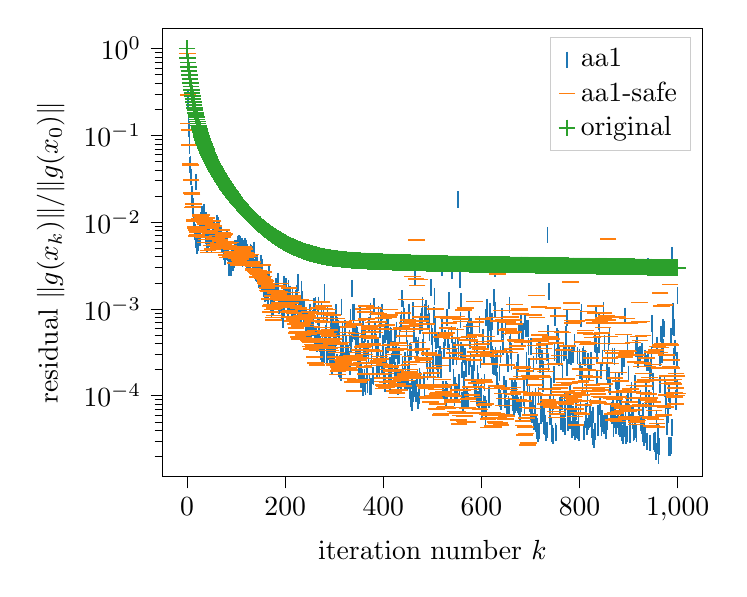
\begin{tikzpicture}

\definecolor{darkgray176}{RGB}{176,176,176}
\definecolor{darkorange25512714}{RGB}{255,127,14}
\definecolor{forestgreen4416044}{RGB}{44,160,44}
\definecolor{lightgray204}{RGB}{204,204,204}
\definecolor{steelblue31119180}{RGB}{31,119,180}

\begin{axis}[
legend cell align={left},
legend style={fill opacity=0.8, draw opacity=1, text opacity=1, draw=lightgray204},
log basis y={10},
tick align=outside,
tick pos=left,
x grid style={darkgray176},
xlabel={iteration number \(\displaystyle k\)},
xmin=-50, xmax=1050,
xtick style={color=black},
y grid style={darkgray176},
ylabel={residual \(\displaystyle \norm{g(x_k)}/\norm{g(x_0)}\)},
ymin=1.16927418743876e-05, ymax=1.71735913919704,
ymode=log,
ytick style={color=black}
]
\addplot [semithick, steelblue31119180, mark=|, mark size=3, mark options={solid}, only marks]
table {%
0 1
1 0.88062612659045
2 0.267059419683147
3 0.132711796458526
4 0.118912387708239
5 0.0766123838845656
6 0.0456578345881652
7 0.0457984381692525
8 0.0332635405949322
9 0.0183234492370433
10 0.0211325678680136
11 0.0143822793915449
12 0.0143667118683201
13 0.0152020347016554
14 0.00974052061586112
15 0.010067182800497
16 0.0077125538926635
17 0.00635993290383208
18 0.0289503331249098
19 0.00683184873896399
20 0.00530730601996308
21 0.00654753843501287
22 0.00583691108113024
23 0.00716996194014418
24 0.00671812280647927
25 0.00721651965235874
26 0.00663584889931062
27 0.00902535580805888
28 0.00994361794311421
29 0.0103739028529308
30 0.0106405211752865
31 0.0122558741874404
32 0.0116223906544444
33 0.0111937717295644
34 0.0129907864065993
35 0.0102486484934572
36 0.00983983394008628
37 0.0090321897701203
38 0.0105108451374985
39 0.00700257570154232
40 0.00878264870447805
41 0.0056743970595196
42 0.00592129711248699
43 0.00695289947981973
44 0.00572604787350734
45 0.00663166763930084
46 0.00664200253220465
47 0.00640220601477367
48 0.00639513822667522
49 0.00614000943742883
50 0.00569587514038626
51 0.00647504035029578
52 0.0068982272496648
53 0.00753568780561355
54 0.00742592506751759
55 0.00820578745685454
56 0.00660999429810427
57 0.00701086050139972
58 0.0076810831467412
59 0.00716480846528039
60 0.0437565058634705
61 0.00982053366815378
62 0.00651014961794608
63 0.00916933791267524
64 0.00684142220799444
65 0.00832630416085653
66 0.00726125717035474
67 0.00603785048219796
68 0.00598825580502338
69 0.00702369787569881
70 0.00578932155230338
71 0.00567358280035529
72 0.00544207072623786
73 0.00551931767145469
74 0.00523930171898409
75 0.00460313209899417
76 0.0043826185162935
77 0.00398352591853258
78 0.00584958216138146
79 0.00477660174759218
80 0.00536315618516896
81 0.00457109357266101
82 0.00639928312548003
83 0.00477559013723789
84 0.00438893698413058
85 0.0032311968233657
86 0.00301802418954063
87 0.00302432015561457
88 0.00357494987805597
89 0.0029768899259427
90 0.00334413365222083
91 0.00407387006879434
92 0.004344048518381
93 0.00342400385603606
94 0.004196456352172
95 0.00387733794437215
96 0.00366440771360846
97 0.00444336398245719
98 0.00499261930844977
99 0.00438297148225908
100 0.00500336704406355
101 0.0047984907561129
102 0.00448744538240539
103 0.00557975630939213
104 0.00432017949780302
105 0.00501363258537246
106 0.00568568389249026
107 0.00452886592472372
108 0.00496949225907471
109 0.00560388430060604
110 0.00403850840905685
111 0.00461542091541021
112 0.00524297288757924
113 0.00383524360914388
114 0.00406972363825661
115 0.0048944252527928
116 0.00493240656687194
117 0.00437096856274377
118 0.00521192236179323
119 0.00494662595124415
120 0.0044342527395882
121 0.00502755765024278
122 0.00370052704685828
123 0.00446960924501284
124 0.00352265572169401
125 0.00383956787104788
126 0.00371144172326907
127 0.00400492425530917
128 0.00363985727683225
129 0.00454674571405529
130 0.00383345064481799
131 0.00437737955766785
132 0.00422256992403102
133 0.00394665785291612
134 0.00327259846618174
135 0.00292627830010974
136 0.00478346432838154
137 0.00292136365679381
138 0.00303309050527722
139 0.00298230262656502
140 0.00320507823085653
141 0.00258897281018183
142 0.00334110488442507
143 0.00254280506221171
144 0.00257783897538322
145 0.00249659224510509
146 0.00250553065456084
147 0.00218348929520186
148 0.00235399852533587
149 0.002118075587612
150 0.00217322531180134
151 0.00336264534347864
152 0.00232724825093654
153 0.00196743669731554
154 0.00302031432268205
155 0.00213732401872564
156 0.00191032984989814
157 0.00170080514067818
158 0.00183996674576633
159 0.00149427210490711
160 0.00221685001380455
161 0.0016524629943479
162 0.00155610289293548
163 0.0016305839293601
164 0.00119913308138806
165 0.00206161807885829
166 0.0013003075823716
167 0.00263342013455849
168 0.0022747404612753
169 0.00172443241453844
170 0.00134372542311667
171 0.00111030583841666
172 0.00100143788328074
173 0.00156798346024885
174 0.00124209686118058
175 0.00102252796424384
176 0.00116542624515848
177 0.00134402631613209
178 0.00132709377713386
179 0.00158285810401715
180 0.00159771098586809
181 0.00181474610454428
182 0.00176200666494737
183 0.00179340669351086
184 0.00170237591059917
185 0.0020620149300891
186 0.0017645407179345
187 0.00120167345684827
188 0.00108981176321967
189 0.00117284482150649
190 0.00110946900524205
191 0.00116428098902788
192 0.00131047623437917
193 0.000950165693870013
194 0.00105698778864171
195 0.00075166617181185
196 0.0012265528332419
197 0.0009727195744828
198 0.00194593929156434
199 0.0012981456728859
200 0.00147799906200473
201 0.0017986435737115
202 0.00149638131196414
203 0.00175376864583263
204 0.0013953202959169
205 0.00106689107742066
206 0.000984064552534715
207 0.00173341192700368
208 0.00109730065940064
209 0.00116276305732744
210 0.00149288586343972
211 0.00115671822215061
212 0.00115532936853066
213 0.00113534150936261
214 0.00104588116128903
215 0.00142703238547731
216 0.00102978258881052
217 0.000827060374843916
218 0.00082646423652145
219 0.00115097552133208
220 0.000843937308568907
221 0.00131159632087299
222 0.00114058815526793
223 0.00125331984721945
224 0.00150004584285097
225 0.000889546165001941
226 0.00200822971321445
227 0.00111060220261369
228 0.00101280092357238
229 0.00100419200107562
230 0.00102625405310878
231 0.00103068006690548
232 0.000796151035945783
233 0.00169448507954627
234 0.0012802372624787
235 0.00101096421933764
236 0.0010514593180265
237 0.000769106316055765
238 0.000936044236138066
239 0.000994585500544825
240 0.000834394959096567
241 0.000804438114774415
242 0.00067240307031609
243 0.000822577405365068
244 0.000541896250766693
245 0.000749243897688352
246 0.000702330432603213
247 0.000700871556716261
248 0.00056642892829653
249 0.000663393951988769
250 0.00060872572629431
251 0.00092487013337408
252 0.000722795926742867
253 0.000516867594703952
254 0.000601806040447485
255 0.00069247881979342
256 0.000775710997382667
257 0.000605766744096367
258 0.000740032078135355
259 0.00107619312740414
260 0.0004802240994277
261 0.000483465195259688
262 0.00108763001949248
263 0.000457665541152112
264 0.000513140686289911
265 0.000401916445710089
266 0.000809486165269262
267 0.000446301361616533
268 0.00110857200949084
269 0.000623200822131878
270 0.000429203837492832
271 0.000393843054185259
272 0.000320459734535668
273 0.000322062485983841
274 0.000946795455602168
275 0.000280849066272545
276 0.000381954642631384
277 0.000299661580682108
278 0.000877216544963201
279 0.000296463983745804
280 0.0015381334337857
281 0.000427020306298132
282 0.00049697563816212
283 0.000528009636768886
284 0.000687107168215085
285 0.000296535541513502
286 0.000876870638803054
287 0.000330255787029818
288 0.000414186060816796
289 0.000322486206541986
290 0.000327343700822624
291 0.000380918822749582
292 0.000300314972902075
293 0.000690487428684165
294 0.000338298007590411
295 0.000219575195766822
296 0.000251498980943146
297 0.000675562466629962
298 0.000311208080721593
299 0.000261473257670395
300 0.000461506934244089
301 0.00039103654129429
302 0.000571722529122399
303 0.000464314183458247
304 0.000903395739508027
305 0.000240823310023623
306 0.000642597653861254
307 0.00023095936307032
308 0.000592173468044887
309 0.0002058749002549
310 0.000503942016268011
311 0.000200351227646498
312 0.000235829096765499
313 0.000336289880981912
314 0.000183295101970626
315 0.0010511484436494
316 0.000328655825777826
317 0.000559177757620055
318 0.000416804543281198
319 0.000276977513966304
320 0.000242961738080702
321 0.000248449237860732
322 0.000602949620205064
323 0.00026034834902031
324 0.000402524133499189
325 0.000262342076319735
326 0.000291341116001117
327 0.000319427738616504
328 0.000309163227316879
329 0.000260798466442711
330 0.000261402733928448
331 0.000462069371507632
332 0.000217585381846818
333 0.000791988989042137
334 0.000392045280635019
335 0.000435101415001501
336 0.00173214502228795
337 0.000514789301205489
338 0.000911285243540485
339 0.000613364577136384
340 0.000559399891887176
341 0.000925660373135914
342 0.000550097507498523
343 0.000431202822597346
344 0.000522287987331832
345 0.000361402767605537
346 0.000491640731558733
347 0.000445069212971436
348 0.00043809364499109
349 0.000262764019264256
350 0.000212810323316365
351 0.000182465753024685
352 0.000838970188012203
353 0.000296991119617957
354 0.000188714887217651
355 0.000151196129550206
356 0.000163258076192774
357 0.000482429693082019
358 0.000124809639008563
359 0.000579111226636032
360 0.00033917141675152
361 0.000139109198198428
362 0.000162395719994393
363 0.000511437478592914
364 0.000126692906495686
365 0.000312701922592335
366 0.000238066043028043
367 0.000168270404649294
368 0.000133957081741498
369 0.000355260308841806
370 0.000286865793609958
371 0.000654121527571338
372 0.000144451402999711
373 0.00012706312544043
374 0.000945036918079355
375 0.000127635959445976
376 0.000264115421665421
377 0.00046818328625877
378 0.000410252478557342
379 0.000171040569438534
380 0.000163936501682512
381 0.00105871648352957
382 0.00046887644532791
383 0.000564113261650227
384 0.000489411632975142
385 0.000410142766169563
386 0.000281277545270906
387 0.000196555211225089
388 0.000298104634076364
389 0.000359222833703895
390 0.000858915333123944
391 0.000220071381381778
392 0.000194519603926591
393 0.000583643857205143
394 0.000264367332762402
395 0.000792750369579617
396 0.000237170917789189
397 0.000227675520619598
398 0.000919049663864369
399 0.000404576593721562
400 0.000284532124090002
401 0.000216033096407785
402 0.000171205897418663
403 0.000509171934238965
404 0.000138112925649431
405 0.000565544690633355
406 0.000295851425306117
407 0.000546921073139425
408 0.000632924295129195
409 0.000629020817426908
410 0.00038268465788806
411 0.000168527209615387
412 0.000447677412901288
413 0.000141067947658343
414 0.000223788226739459
415 0.000491904588724157
416 0.00015999613162166
417 0.000479357696552681
418 0.000249568187841198
419 0.000330027988076314
420 0.000341717613167043
421 0.000287525280250857
422 0.000294825875913912
423 0.000200518150007476
424 0.000476568018358342
425 0.000198507688747734
426 0.000326240761077961
427 0.000573934896902832
428 0.000179386980736122
429 0.000260224404481205
430 0.000125927966082378
431 0.000161545800305176
432 0.000292582905189877
433 0.000510353315423746
434 0.000152924573335327
435 0.000689002227778827
436 0.000148778215101121
437 0.000753006186439019
438 0.00130923819438795
439 0.000221241365342867
440 0.00016826983320054
441 0.000998659986129475
442 0.000832051529757328
443 0.000148219204729308
444 0.000254149575524667
445 0.000200386887093018
446 0.000140803167008187
447 0.000517464160216201
448 0.000141818028438102
449 0.000349381352371979
450 0.000178274441867215
451 0.000150219327551026
452 0.000924701585028815
453 0.000235510528938088
454 0.000321825147677994
455 0.000113084434235379
456 0.000317145414675904
457 9.15762238904513e-05
458 0.00014913850214458
459 8.37069708247196e-05
460 0.000960822105799616
461 0.00010476649481604
462 0.000120785162236908
463 0.000520880956536973
464 0.000120699965770933
465 0.00237832341389613
466 0.000385862274987618
467 0.000106140918590163
468 0.00014141350764995
469 0.000349377005139235
470 0.000163400060101149
471 8.79890824382415e-05
472 0.00037928762517198
473 9.8771740913491e-05
474 0.000168375423508515
475 0.000643888716931864
476 0.000150987438467291
477 0.000711870795323765
478 0.000832892617004085
479 0.000701605307536607
480 0.00109451204096964
481 0.000358677134596515
482 0.000422381678164973
483 0.00015099275761082
484 0.000115763534034753
485 0.000915998166190405
486 0.00100193224471606
487 0.00100322701943947
488 0.000806989243551718
489 0.000270103785068478
490 0.000190974527582287
491 0.00070840176239361
492 0.000893405804071408
493 0.000722480191939136
494 0.000535588740073411
495 0.000201577714293995
496 0.000208775886141261
497 0.00175785483380978
498 0.000522834104435336
499 0.000477272482984069
500 0.000398981044747815
501 0.000230071606490054
502 0.00016301394593183
503 0.000833310728215711
504 0.00140100126428793
505 0.00064065015829333
506 0.000523600439369282
507 0.000431565663027498
508 0.00027063920575643
509 0.000245226719393586
510 0.000245300616885994
511 0.000198900674026172
512 0.000436281919965663
513 0.000255180770379189
514 0.000267984649184985
515 0.000296395719264705
516 0.000249820698771424
517 0.000198630443190848
518 0.000264181461852722
519 0.00295871836784998
520 0.000650686957434978
521 0.000113295419059573
522 0.000117417481911139
523 0.000118544714622812
524 0.000334674273784599
525 9.68743594393689e-05
526 0.000460708157290657
527 9.26073972866323e-05
528 0.000118179634415104
529 9.11502456432665e-05
530 0.000795033858331672
531 0.000111552585704013
532 0.000423834964771232
533 0.00047932995558153
534 0.00124829136645139
535 0.00031828167875999
536 0.000233980392505104
537 0.000105279852017171
538 0.000108125781427492
539 0.00050457992682477
540 0.00275145585857867
541 0.000393146758105575
542 0.000279949396043083
543 0.000162402961788151
544 0.000334196035231025
545 9.52722228937527e-05
546 0.000133392400958443
547 0.0003582675595174
548 0.000112089385133099
549 0.000282456251662732
550 0.000109228774484931
551 0.000485331434100235
552 0.0183092270629337
553 0.000339781530431518
554 0.000142910138860247
555 0.000125750747344865
556 0.00218137494066499
557 0.000743030992011354
558 0.00121080126307564
559 0.000335443028334154
560 0.000197509760929907
561 8.80036940208062e-05
562 8.31028957835042e-05
563 0.000298529551311007
564 0.000154867253268838
565 0.000115158849852101
566 9.26420173418006e-05
567 0.000282177026794794
568 0.000207038978413545
569 9.27289289720993e-05
570 9.80027535545189e-05
571 0.000539153784538007
572 8.64294785445242e-05
573 0.000584133734881034
574 0.00021768423226004
575 0.00076111520017845
576 0.00081393860739857
577 0.000430248704570802
578 0.000263747408257056
579 0.000636820042496481
580 0.00017902756848466
581 0.00016825260259551
582 0.00054977777087777
583 0.00017983812676127
584 0.000162214135609174
585 0.000238655710419265
586 0.000413407821881765
587 0.000118478467513968
588 0.00011928927844548
589 0.000117699564446031
590 9.76974795889388e-05
591 0.000353895474280154
592 0.000180939446456618
593 9.13516995696516e-05
594 0.000145280938522105
595 8.81596581509413e-05
596 0.000661425015801645
597 9.90670160717836e-05
598 0.000260805318434799
599 0.000107408820709716
600 0.00012952780143102
601 6.87525488693663e-05
602 6.61046951681657e-05
603 0.000473725882031681
604 8.18629428832592e-05
605 0.000283765841090944
606 0.000141134801139903
607 7.87417637980559e-05
608 5.72287632837149e-05
609 0.000792397372571686
610 7.08741614694551e-05
611 0.00105030641530863
612 0.000915270094248199
613 0.000602355684204087
614 0.000439004086761969
615 0.00010106909483609
616 9.05103647176169e-05
617 0.0009289508080779
618 0.000702894587417223
619 0.000452617967625511
620 0.000335763556156798
621 0.000297213364796338
622 0.000715753871940549
623 0.000224408617708311
624 0.000277226405662424
625 0.00021681568151778
626 0.00135009243188371
627 0.00294274149721493
628 0.000975233267841704
629 0.000293278794027776
630 0.000210887488743452
631 0.000148972761021735
632 0.000260578279598873
633 0.000151337561384946
634 0.000620995084857437
635 0.000113186233024407
636 9.82926608549387e-05
637 0.000183998690871855
638 9.32717194705971e-05
639 0.00029836624246222
640 8.59859476771103e-05
641 0.000525350553633495
642 0.000815808544949604
643 0.000571733993503706
644 0.000363894097777277
645 0.000460841053651512
646 0.00013477670896835
647 0.000113508209996672
648 8.88043763271424e-05
649 0.000621963395015074
650 0.000121958436954009
651 0.000280513044655304
652 7.24667067287672e-05
653 0.000245903338792427
654 0.000236748950294167
655 7.87532464734657e-05
656 7.56338053079111e-05
657 0.00110756534428429
658 0.0003947493563684
659 0.000415282488120507
660 0.000327573201473241
661 0.000244791638879014
662 0.000124252049397435
663 0.000120325167674289
664 8.26342587152485e-05
665 0.000116858710437787
666 7.11308908462578e-05
667 7.24361938112377e-05
668 7.85634718973356e-05
669 0.00012974004647324
670 0.000114556503205308
671 9.91354145128577e-05
672 0.000196257854443782
673 8.2829662067403e-05
674 0.00024416941478725
675 7.7772824920215e-05
676 0.000539430349684627
677 7.37382736771424e-05
678 6.40875391027926e-05
679 6.87089000587229e-05
680 0.000675577628135045
681 8.05404942164348e-05
682 0.000668488493256458
683 0.000481451781939598
684 0.000528662190707196
685 0.000547802979288357
686 9.59124066996173e-05
687 0.000125082504772745
688 7.23287500321117e-05
689 0.000705908258950245
690 0.000701644596472898
691 0.000598013171270253
692 0.000257779432650189
693 0.000162274609750219
694 0.000122937781277374
695 0.000596532411310105
696 0.000370881610490068
697 0.000217660186943201
698 0.000104490324062498
699 8.10758077468095e-05
700 6.28329690975217e-05
701 0.000367333655505493
702 6.7550835604602e-05
703 6.00853477350931e-05
704 9.14071928188384e-05
705 8.8659070356765e-05
706 0.000232492766671061
707 5.02208842394871e-05
708 5.16645255302409e-05
709 6.1950137750862e-05
710 9.75410047810445e-05
711 4.77904710184863e-05
712 0.000291185846541324
713 3.96836473992065e-05
714 4.40140576360549e-05
715 3.68969051044149e-05
716 0.000101681185379643
717 3.93755611710588e-05
718 0.000351939274732625
719 0.000226531448398604
720 0.000368267589493695
721 8.54458395546198e-05
722 5.86237146199323e-05
723 0.000268998413750292
724 6.15144465774338e-05
725 0.000139181069415584
726 0.000199801949770532
727 5.77102014005076e-05
728 4.50857348609842e-05
729 4.82649903652228e-05
730 4.34461507771151e-05
731 3.78895023300852e-05
732 3.69606447733908e-05
733 0.000316397595338114
734 4.02743315707336e-05
735 0.00708386703051943
736 0.000525282380409875
737 0.000239785920501091
738 0.00158330255401215
739 8.28830932269906e-05
740 5.69088949720357e-05
741 0.000105886076159175
742 0.000129691676825741
743 4.42786828857476e-05
744 3.68699302696608e-05
745 7.44426479495348e-05
746 3.44417739602511e-05
747 8.48096723663321e-05
748 0.000174426978105773
749 0.000315725323796696
750 0.000796926181243549
751 3.85934046532337e-05
752 3.71926021343334e-05
753 0.000287599330129436
754 0.000489008610008963
755 0.000293543273617963
756 0.000418639584775768
757 0.000455322845143257
758 0.000273209009627444
759 0.000311111524452053
760 7.85084318377548e-05
761 5.01984573963125e-05
762 5.01729148847849e-05
763 0.000275708237231308
764 8.48753473328383e-05
765 0.000189669802446943
766 4.79385728825456e-05
767 0.000320362426720008
768 0.000311001729199418
769 9.09947660113283e-05
770 7.1386550548262e-05
771 4.42020402852983e-05
772 0.000327715771382394
773 0.000504700781998756
774 0.000787063639315023
775 0.000212869976408156
776 7.11895870124834e-05
777 4.9434482026624e-05
778 0.000288636692030955
779 7.51592865547128e-05
780 0.000106703009619937
781 5.13198119304843e-05
782 0.000278540451725951
783 7.43223463973757e-05
784 0.00029467008338004
785 4.08453822983595e-05
786 6.0665267589356e-05
787 4.25462126890362e-05
788 0.000293256734355973
789 5.56111699521796e-05
790 0.000408060815155264
791 3.88398977464471e-05
792 5.09044505024274e-05
793 6.54708761425043e-05
794 7.33087963311323e-05
795 4.10515360850459e-05
796 0.000290139250748951
797 3.93222258398991e-05
798 6.00524652380996e-05
799 3.73026063831589e-05
800 0.000277521902625184
801 0.000193812583952641
802 7.38456437582568e-05
803 0.000771740392702251
804 0.000910649240800965
805 0.000174118335254387
806 0.000132661063468824
807 0.000283039020431683
808 0.000301388807760239
809 3.80816186300302e-05
810 4.14985320244832e-05
811 0.00027224336996821
812 5.26924379865212e-05
813 6.5883576313732e-05
814 0.000138510654518455
815 4.38017741006617e-05
816 9.17199857146733e-05
817 0.000249398617024111
818 5.06605607086042e-05
819 0.000185824154484852
820 5.33449314765947e-05
821 6.16203088436694e-05
822 7.33063575600403e-05
823 0.000253035284647653
824 5.40257750798496e-05
825 4.02934590777161e-05
826 4.356918789802e-05
827 3.3443348672294e-05
828 6.00868286176488e-05
829 3.1259697727584e-05
830 3.11818629193961e-05
831 0.000399048545599082
832 3.84371327750992e-05
833 0.00038912814117276
834 0.000868727241037482
835 0.000290438112152506
836 0.000160210552650929
837 6.34531745066928e-05
838 4.31131902480539e-05
839 0.00038576402671035
840 0.00071409236742639
841 0.000536996152966174
842 7.51235683135645e-05
843 5.44816605354515e-05
844 0.0001925434142225
845 4.22831249573684e-05
846 5.46298544885027e-05
847 0.000271493048215098
848 4.79127924117538e-05
849 0.000956581673217117
850 4.47090871830938e-05
851 0.00039768450070534
852 5.02171883391865e-05
853 4.0328952320723e-05
854 3.90295791385111e-05
855 0.000190257753624255
856 5.01211367596968e-05
857 0.000265396501166797
858 0.000170811799740454
859 0.000415936909387756
860 0.000170047697654229
861 0.000482536352422079
862 0.000127496741461558
863 6.68992400831016e-05
864 6.13085928073361e-05
865 6.79039602495936e-05
866 5.91026968527367e-05
867 0.00028754611831741
868 7.70653813878685e-05
869 4.13826754395406e-05
870 5.24645015415738e-05
871 0.000283678348408708
872 6.42264323349474e-05
873 0.000147682128582276
874 4.51631309406759e-05
875 4.69118488653492e-05
876 9.89398702534488e-05
877 0.000118968497751118
878 5.27260475778691e-05
879 0.000109170715306072
880 0.000147813094407968
881 4.38419627829579e-05
882 7.61888510244399e-05
883 4.16142174683562e-05
884 9.11565609898371e-05
885 4.87389510066606e-05
886 0.000217026743424976
887 3.7227925472975e-05
888 5.89405410213548e-05
889 3.41322701815432e-05
890 0.000269997365923168
891 4.53976455294064e-05
892 0.000828519149413406
893 4.19821182035674e-05
894 6.89335112008766e-05
895 3.47983344883009e-05
896 8.21578632189091e-05
897 3.60413398704672e-05
898 0.00039898902346958
899 9.68108242679897e-05
900 0.000178146684248991
901 6.42795246523024e-05
902 4.97595115311093e-05
903 3.53758690751953e-05
904 4.99568635279337e-05
905 0.000101827074470161
906 0.000115234226209368
907 6.24044539479393e-05
908 5.19377171575707e-05
909 6.19537534891676e-05
910 3.70027309282226e-05
911 3.80906559335566e-05
912 3.90226120317994e-05
913 0.000138375394809368
914 4.03401908583465e-05
915 0.000345710681138685
916 3.64282864996695e-05
917 0.000406431079954634
918 0.000306774771272123
919 0.000256757611002944
920 0.000290496833982625
921 7.41579790421091e-05
922 5.98173578244262e-05
923 0.000296587812776544
924 9.42070550248397e-05
925 4.83661488273109e-05
926 4.45737913131518e-05
927 0.000325658786546751
928 4.97131478777439e-05
929 3.64489206694711e-05
930 6.6205186727608e-05
931 3.24059467485963e-05
932 4.42681029148004e-05
933 0.000269978093639713
934 3.51291050479748e-05
935 0.000125441774269159
936 8.9735943057783e-05
937 2.96790105555966e-05
938 0.000237531103924255
939 0.0030606226280413
940 0.000240473707827149
941 6.51467633250065e-05
942 9.3262474675962e-05
943 2.85554939019978e-05
944 0.000185562231617544
945 7.05401666924074e-05
946 0.000210358516047198
947 0.000301292310342512
948 0.000675466627015311
949 0.000437830221902421
950 0.000146729645538908
951 9.83999779963238e-05
952 2.96967271843776e-05
953 2.79840988655458e-05
954 3.08320306340588e-05
955 2.35563865469288e-05
956 2.27846796100938e-05
957 5.49371793541413e-05
958 0.00038573786603203
959 2.67719959968795e-05
960 3.8060965756197e-05
961 2.00806371202515e-05
962 2.59333697728444e-05
963 0.00027729650616627
964 0.000133221358983568
965 0.000272392401643945
966 0.000513791778960658
967 0.000468515471391678
968 0.000298595350031632
969 0.000397915226685158
970 0.000612033633823769
971 0.000359988295874198
972 0.000586303149714051
973 0.000135270030367501
974 0.000120903888197975
975 7.11830661148745e-05
976 8.7094874941505e-05
977 4.67220122530343e-05
978 4.40650963596126e-05
979 4.62379945613361e-05
980 6.01875551853892e-05
981 2.50185912426794e-05
982 0.000105966860618905
983 2.65261186288677e-05
984 8.8305552738161e-05
985 2.52162398758641e-05
986 2.67090712608808e-05
987 0.000484448544059626
988 4.31383530850465e-05
989 0.0041742289898428
990 0.000932129333873093
991 0.000627417817765045
992 0.000280659945229607
993 0.000607205406040072
994 0.000354892952158724
995 0.000176941609806096
996 9.4200581780974e-05
997 8.4596686139162e-05
998 0.00025559859162354
999 0.000123923617757224
1000 0.00141640321340469
};
\addlegendentry{aa1}
\addplot [semithick, darkorange25512714, mark=-, mark size=3, mark options={solid}, only marks]
table {%
0 1
1 0.877894606439485
2 0.289703339709453
3 0.136966689962867
4 0.115686719881149
5 0.077564770600522
6 0.0466186216299358
7 0.0458348885090002
8 0.0307301213460682
9 0.0216797688217219
10 0.0209060568152221
11 0.0148013037116318
12 0.0150344938419235
13 0.0162486098680063
14 0.0105720314405484
15 0.0103095036734539
16 0.00872877922624474
17 0.00846219028065182
18 0.00696720872650668
19 0.00814202818006118
20 0.007060770841929
21 0.00775810491254261
22 0.00759712521402947
23 0.00829578918407582
24 0.00777237124698348
25 0.0109103575978808
26 0.0120631270760584
27 0.0116778363220235
28 0.0122838487336838
29 0.0119330495210497
30 0.0121225765988504
31 0.0111677705010698
32 0.00863257184358561
33 0.0110757736523576
34 0.00672102875730537
35 0.0105954377864458
36 0.00999237667031385
37 0.00958109295253858
38 0.00582424886823937
39 0.0111029652942849
40 0.00630369550426379
41 0.00891694444929188
42 0.00799696214338695
43 0.00470112995528773
44 0.00445544596566891
45 0.00959329170385474
46 0.00799730792024437
47 0.00796884296195243
48 0.00751827771606452
49 0.00855753042602637
50 0.00538122913201703
51 0.00955864516685513
52 0.00488292266606908
53 0.0102497545788908
54 0.00899481546557163
55 0.00635570719366443
56 0.00798027600645114
57 0.00752457900073936
58 0.00543063052777348
59 0.00667285679518547
60 0.00663073838287171
61 0.00657078316139845
62 0.0070192070411689
63 0.00512692495411922
64 0.00564751935484584
65 0.00747252823292068
66 0.00632212644624665
67 0.00603996784272789
68 0.00447744271829885
69 0.00539641331754285
70 0.0052830272002638
71 0.00808192761557723
72 0.00761800932720508
73 0.00679268948607891
74 0.00709917146683917
75 0.00543811714635831
76 0.00591251318576737
77 0.00726542528790514
78 0.00591308455078388
79 0.00570163458625284
80 0.00418295572573617
81 0.00534081490961109
82 0.00390399242159842
83 0.00536064137014447
84 0.00537925880733406
85 0.00571952876084791
86 0.00511912065167553
87 0.00502343514518255
88 0.00400044365732535
89 0.00582267929942426
90 0.00514594930102218
91 0.00483836354858627
92 0.00449801736869121
93 0.004394355628966
94 0.0041825067930457
95 0.00424464266044887
96 0.00414336856176813
97 0.00404831758707732
98 0.00394608566996731
99 0.00341150261648547
100 0.00383817474803046
101 0.00434752733351775
102 0.00390800646022026
103 0.00381765038440836
104 0.00387205545227395
105 0.00321554379592034
106 0.0036133952831117
107 0.00378426238604929
108 0.00347078124489655
109 0.00371093236227446
110 0.00380336686145697
111 0.00399218171928952
112 0.00400640286912332
113 0.00476275270050209
114 0.00455781278399359
115 0.00523523945048258
116 0.00511115860650312
117 0.00403975804776252
118 0.00494397359190479
119 0.0043879477550835
120 0.00394989148464235
121 0.00433060383089522
122 0.00408581402495429
123 0.00352140282752212
124 0.00409748964964382
125 0.00318306732427893
126 0.00327513287607117
127 0.00403116610833206
128 0.00329770227708541
129 0.00424243569745993
130 0.0033863971374106
131 0.00344185925926464
132 0.00340782374305914
133 0.00344631775115739
134 0.00291031387233303
135 0.00312475572887464
136 0.00282769649169053
137 0.00308987621855833
138 0.00284189753956279
139 0.00269831611373977
140 0.00274881858293586
141 0.00268093342024641
142 0.00273136832536782
143 0.00257519706126513
144 0.00233437848597531
145 0.00276330374071476
146 0.00251387461644258
147 0.00229389283216216
148 0.00229776353697243
149 0.00239543375777066
150 0.00236850118898586
151 0.00259550123333356
152 0.00233154787291375
153 0.00258187169752235
154 0.00228126749582381
155 0.00319847508949422
156 0.00266637017226281
157 0.00235571468016403
158 0.00218119280979641
159 0.00200231671863567
160 0.00210476590869631
161 0.00194354204562337
162 0.00193448043848406
163 0.0017320530377594
164 0.00162355642061774
165 0.0016137741141747
166 0.00163432821549295
167 0.00184946680993395
168 0.00130855483918686
169 0.00107989393057793
170 0.000914749719002762
171 0.00111998830128319
172 0.00106786464340466
173 0.00141787418910669
174 0.000987389010420013
175 0.000795826912033948
176 0.00075106090574862
177 0.000837745371133409
178 0.00102871770901469
179 0.00151405139400739
180 0.00132243466546985
181 0.00105039419484964
182 0.00142928052057686
183 0.00160302824522395
184 0.0018308382724438
185 0.00139249533053556
186 0.0013310375837249
187 0.00148201991659137
188 0.00158700119286058
189 0.0011679106951513
190 0.00196951351289245
191 0.00117040556258545
192 0.00124775529519674
193 0.001106402593194
194 0.00140931143097601
195 0.00126184984489658
196 0.00142141628720772
197 0.00127306333031224
198 0.00109199265336424
199 0.00129387694272908
200 0.0010409612344148
201 0.00128372847665341
202 0.00125246022917183
203 0.00124942158240325
204 0.00110363388896551
205 0.00108200022489353
206 0.00126259385297863
207 0.000921441494813341
208 0.00172773882083078
209 0.000808004769321901
210 0.000939022548502135
211 0.00116208367064847
212 0.000800064238031804
213 0.00154811142168859
214 0.000730090432775652
215 0.00140585309444178
216 0.00132954413174443
217 0.00107214461630229
218 0.000903244752462089
219 0.000761526740858747
220 0.000668225457332414
221 0.000809600518968417
222 0.000598750942690626
223 0.000524942912447542
224 0.000542847494240386
225 0.000700219892452348
226 0.000475197748827622
227 0.00101909731169571
228 0.00063656945524744
229 0.000446419417511486
230 0.000548028269636186
231 0.00125695194835336
232 0.000539635192817254
233 0.000832042324930032
234 0.000630019170363417
235 0.000690121735780653
236 0.000499243933290089
237 0.000984054193643035
238 0.000461970996378018
239 0.00124844244905978
240 0.00076506392537989
241 0.000661236696694442
242 0.000626545952017239
243 0.000540265093581071
244 0.000851821163793297
245 0.000838063733702634
246 0.000800236022436023
247 0.000512088648665575
248 0.000431274733464491
249 0.000425775791706272
250 0.000925357684593416
251 0.000369357730144304
252 0.000416756089843576
253 0.000346153577562313
254 0.000625306484384803
255 0.000387593020076602
256 0.000722755093078626
257 0.000365584486741062
258 0.000384538733531665
259 0.000282515088744411
260 0.000277060340953637
261 0.00056211673096337
262 0.000236834789403317
263 0.000900955502872636
264 0.000448653944466875
265 0.00022739872175769
266 0.00033046718811348
267 0.00103254411912716
268 0.00073715084567261
269 0.00053165918947213
270 0.000790956665902263
271 0.000383027766587246
272 0.000350472301340912
273 0.00120429304217519
274 0.000359155299254421
275 0.00120971987010433
276 0.000609832239091026
277 0.000711704376027425
278 0.00108283316361779
279 0.000861795753518191
280 0.00100032317370686
281 0.000431577080456127
282 0.000538138782242744
283 0.000413989248439235
284 0.000905112877939456
285 0.00036795518963762
286 0.000981719591743908
287 0.00051371427615728
288 0.000520000542920283
289 0.000488032400477189
290 0.000576019198606225
291 0.000352086832593338
292 0.000330896197831503
293 0.000444832148333863
294 0.000440799665191117
295 0.000393424431411691
296 0.00085522343341354
297 0.000417862615273519
298 0.00023499631077584
299 0.000447499145935489
300 0.000456812392259322
301 0.000226755991434345
302 0.000277968731002611
303 0.000402941178722278
304 0.000313513074859212
305 0.000773820773774064
306 0.000260732022856512
307 0.000174874031881135
308 0.000193518170202467
309 0.000213265599168317
310 0.000391111671000064
311 0.000202732715486277
312 0.000391433476027691
313 0.000709982961605735
314 0.000217206452275624
315 0.000409799395775428
316 0.000715239043517953
317 0.000254329648422818
318 0.000359754569867382
319 0.000244838247350088
320 0.000707912663061081
321 0.000267768339456825
322 0.0004931833941887
323 0.000233256115029209
324 0.000268117229444431
325 0.000265327951753283
326 0.000536830635343029
327 0.000158456948173082
328 0.000619960845095732
329 0.000201588928366427
330 0.000210908662109225
331 0.000198313963248005
332 0.000274952960232841
333 0.000224578570105474
334 0.000286393673927066
335 0.000285996722204444
336 0.000231709883388594
337 0.00014292257040589
338 0.000143707174320906
339 0.000653725872346367
340 0.000113203747021466
341 0.000677661541384427
342 0.000286021327321358
343 0.000151203875919775
344 0.000142654866805826
345 0.000520101701519167
346 0.000142068114295848
347 0.000314804731355897
348 0.000736143027318938
349 0.000257526055949012
350 0.000142633068650523
351 0.000334492709043451
352 0.000315523229444082
353 0.000482775694327576
354 0.000270156249347707
355 0.000236083629595065
356 0.000151306947459892
357 0.000643717219262203
358 0.000365226402488284
359 0.00100178529603653
360 0.000376969307892103
361 0.00021517986730577
362 0.000298856364584001
363 0.000920969548725775
364 0.000177084225204292
365 0.00108830640808058
366 0.000762916132297277
367 0.000393367874154942
368 0.000470846598210387
369 0.000268614181959394
370 0.000487515481983321
371 0.000590544988757234
372 0.00061873204192951
373 0.00077601016892165
374 0.000540728963198014
375 0.000458446261571949
376 0.000336876572068825
377 0.000222849054041617
378 0.000396980194146801
379 0.000699736592724877
380 0.000239603934205821
381 0.00101984476655527
382 0.000326294938638784
383 0.000534382271716716
384 0.000704089453256901
385 0.000910507463750653
386 0.000635807693043793
387 0.000860448219782881
388 0.000379597647155051
389 0.000251650686874722
390 0.000709870489594189
391 0.000867071671581678
392 0.000234578481101185
393 0.000283233417917991
394 0.000179238798122716
395 0.000265590319530456
396 0.000584131277906976
397 0.000160500877166524
398 0.000145737979974312
399 0.000121348644709796
400 0.000789484902629216
401 0.000133307930306875
402 0.000225500479095282
403 0.000129845212006664
404 0.000577642553203938
405 0.000180770421691845
406 0.000648232108615523
407 0.000126790522753001
408 0.000127240569748731
409 0.000143565117527758
410 0.00081345275668809
411 0.000200409889023289
412 0.000159794092088971
413 0.000855032867125153
414 0.000981102867777702
415 0.000386096660875827
416 0.000214000583514533
417 0.000192925967709191
418 0.000579060602017232
419 0.000146795890370383
420 0.00012811041175124
421 0.00029769018823205
422 0.000113113866825684
423 0.000347172527006813
424 0.000133888552799799
425 0.000337942582957822
426 0.000196624737572145
427 9.50911103267939e-05
428 0.000106880971405469
429 0.00013752197437934
430 0.00013670342091348
431 0.000405957958488773
432 0.000117548491531794
433 0.0001144456417313
434 0.000346230444275011
435 0.000222972865169888
436 0.000153268327291764
437 0.000600756247157473
438 0.000164682311487959
439 0.000159510953266039
440 0.000900923265926354
441 0.000129295845492851
442 0.000379811017444807
443 0.000486601521135257
444 0.000168915709694353
445 0.000179001111228462
446 0.00127978929392418
447 0.000149965300756363
448 0.000548790235803175
449 0.000690994725883481
450 0.000744020271505173
451 0.000577917996992941
452 0.000228006177251979
453 0.000200096529682191
454 0.000186252449675909
455 0.000639912295515272
456 0.000282002240675366
457 0.00017076526870009
458 0.000246045428501757
459 0.00236271084255209
460 0.000717516117452268
461 0.000165588417312559
462 0.000178042130964081
463 0.000158636359185916
464 0.000625781390189861
465 0.000336856775970814
466 0.00128907596049261
467 0.00221446964317629
468 0.0062810212696744
469 0.00186353573692678
470 0.000669642859793046
471 0.000411086718817142
472 0.000584798115240567
473 0.00321624051837998
474 0.00218823624019651
475 0.00106606362196916
476 0.00080664780361563
477 0.000721784785215916
478 0.000589654142375266
479 0.000343192769527942
480 0.000272083624075807
481 0.000259483637378634
482 0.000240165332421834
483 0.000276056607028445
484 0.000133439785209826
485 0.00026548601455282
486 0.000129346018477658
487 0.000122380136685368
488 0.000668616652377087
489 9.6405175740985e-05
490 0.000165525335912858
491 9.30096622905409e-05
492 9.81735292121759e-05
493 0.000310513414765852
494 0.000297887652562704
495 0.000525679211699075
496 8.51319565124401e-05
497 0.000180840882795744
498 0.000181551617793571
499 0.000161501293986108
500 0.000130599801302379
501 0.0002930499311776
502 9.87421744802559e-05
503 0.000209728072505807
504 0.000126602751199427
505 9.3227167032162e-05
506 0.000989384685642489
507 0.000117950605960822
508 0.000130591198296955
509 6.99441480461105e-05
510 0.000104826972087567
511 7.96855330710459e-05
512 0.000106673552133268
513 0.000100322466452424
514 0.000133529986664563
515 0.000126441217128088
516 0.000223579881565483
517 5.97980553543299e-05
518 0.000476848780724906
519 6.22421365224096e-05
520 0.000807990087193847
521 0.000153412441266866
522 0.000124863411322413
523 0.000110837337303756
524 0.000134169397473418
525 7.24536987590091e-05
526 0.000504762603238983
527 7.42921306111973e-05
528 7.49913336448289e-05
529 0.00010533541881287
530 0.000526883205143519
531 0.000598452677810402
532 7.11741762306483e-05
533 0.000783851085851949
534 0.000682587067674964
535 0.000349206837632365
536 0.000131952530351598
537 0.000272770971316903
538 0.000105393860382515
539 0.000454795168998586
540 8.95768524402729e-05
541 8.48936322947705e-05
542 0.000790023879698249
543 9.95118228265581e-05
544 6.22498383107504e-05
545 0.000312002208141252
546 7.32645894572985e-05
547 6.56771658735794e-05
548 0.000578540258001423
549 6.60009879895909e-05
550 0.000817575476730826
551 6.47439520082863e-05
552 0.000117217867249672
553 5.24198208377643e-05
554 4.7141371766923e-05
555 0.000468585615350359
556 5.90761890162488e-05
557 0.00076329856983026
558 0.00038249512099729
559 0.00071657991881031
560 0.00046740781619908
561 0.000263818152515768
562 0.000116606923202111
563 0.000260680434769733
564 0.00097718979582755
565 5.81137183521544e-05
566 5.03728023998097e-05
567 0.00102703901974892
568 5.01476040107478e-05
569 0.000442024891971808
570 0.000290480952696063
571 4.93857689367797e-05
572 7.24644170948913e-05
573 9.19608876233126e-05
574 6.3165944848831e-05
575 0.000477733580558934
576 0.000440048897814498
577 0.000286240772484082
578 0.000126046069532477
579 0.000117826167676102
580 0.000628724433447269
581 0.000101136501999119
582 0.000150858748146319
583 9.5142664309416e-05
584 0.000388834019600584
585 0.000258564121290462
586 0.00121902609062892
587 0.000320544472801686
588 0.000500561791380486
589 0.000708074435686549
590 0.000141176393748121
591 0.000125794485918472
592 0.000363250796618307
593 8.57283292460823e-05
594 0.000420542343025171
595 7.12247276575633e-05
596 0.000294873441077592
597 6.94396939420656e-05
598 0.000343308848562856
599 0.000346043009640185
600 0.000321338328058872
601 0.000394698886362115
602 0.000283632494663744
603 0.000767033498044257
604 0.000152376759886022
605 7.85985119210688e-05
606 0.000143847622400581
607 6.30482399244927e-05
608 0.000291869186039454
609 8.07513477355563e-05
610 0.000479109296921328
611 6.06451740348813e-05
612 0.000288310050030368
613 5.40788836618133e-05
614 0.000306315011933216
615 4.29365903227088e-05
616 0.000231998128379932
617 5.9679172317357e-05
618 6.15391370412611e-05
619 5.59417571230854e-05
620 6.05144024716897e-05
621 0.000121019605519609
622 4.50884817262714e-05
623 6.30875234057526e-05
624 4.34846899327424e-05
625 4.34261258947146e-05
626 0.000285929187818035
627 0.000793700777793163
628 4.97526774878285e-05
629 0.00042547207219122
630 4.77678031681786e-05
631 0.000128684816602138
632 6.24302447804804e-05
633 0.00253069948825353
634 0.000327388289283276
635 0.000723771642132804
636 5.57740841231507e-05
637 4.84613294828205e-05
638 4.86495772713001e-05
639 0.000318222105176347
640 4.62778519327564e-05
641 0.000955315800102998
642 0.000122454374893291
643 0.000105653126777851
644 0.00074411758501709
645 7.69130127823191e-05
646 9.30447744068102e-05
647 0.000319344521740563
648 6.02145957661981e-05
649 5.4216628726166e-05
650 0.000568152734972319
651 5.8170406888172e-05
652 0.000225120916264892
653 0.000703786617128335
654 0.000744718465741962
655 0.000581957491823746
656 0.000563936094756432
657 0.00011735769665564
658 0.000315597329096135
659 0.000519741540312853
660 0.000800299155481202
661 0.000954943305215709
662 0.000344057366286921
663 0.000124737916488114
664 0.000104545818412633
665 0.000545196817726427
666 0.000746413802161257
667 0.00112630852402408
668 0.000672781303775228
669 0.000440576505067994
670 0.000344246541016318
671 0.000425494557777845
672 0.00305251219365574
673 0.000377075780468636
674 0.000155587323376556
675 9.03738390360205e-05
676 0.000109892291467815
677 0.000972494820240186
678 0.00100358592386914
679 0.000868712738372171
680 0.000887850517805224
681 0.000207211110384684
682 0.000166105829005737
683 0.000414662248240864
684 0.000212468326653512
685 5.142500063462e-05
686 4.51781152270751e-05
687 8.67540396968966e-05
688 3.5034808902788e-05
689 0.000193308584965267
690 4.32800399172121e-05
691 3.65857698563105e-05
692 5.56810236353806e-05
693 7.27997193353e-05
694 2.71782332809766e-05
695 0.000423418075298344
696 2.87316545676785e-05
697 2.80553646809837e-05
698 0.000167956468773396
699 6.03449409477171e-05
700 0.000159975371835723
701 0.000103778169598314
702 0.000101954961460663
703 0.000106599243517321
704 7.09969505812178e-05
705 0.000107627510829846
706 0.000101727598667535
707 0.000845902180600157
708 0.000106424926477167
709 0.000132446443274953
710 0.000380371573431851
711 0.000153321667069807
712 0.00142715761127987
713 0.000796494150213027
714 0.000378417508947015
715 0.000205262108301104
716 0.000263896811339518
717 0.001044478215844
718 0.00049875893368588
719 0.000453678949277377
720 0.000427348075691435
721 0.000307319448030468
722 0.000203229600209175
723 0.00016760834103886
724 0.000163799160469586
725 0.000166915570532397
726 0.00034952477118733
727 0.000102315156770588
728 0.000393762569267434
729 0.000103470795639482
730 0.000190481651795946
731 8.00310069269549e-05
732 0.000550061808846494
733 0.000118576227413747
734 0.000228925189900489
735 8.10674252414275e-05
736 8.92014538985763e-05
737 7.82195797744365e-05
738 0.000269332484701555
739 8.1886662719649e-05
740 0.000471292629430493
741 8.50933168895152e-05
742 7.35399983899287e-05
743 7.37293483434121e-05
744 0.000451902484138743
745 0.000118919041612396
746 0.00103162173691351
747 7.33796607643461e-05
748 8.13374635454932e-05
749 8.42641516203045e-05
750 0.00023364798555988
751 6.58497696468284e-05
752 0.000408007866486094
753 5.61799983894408e-05
754 6.13435404183162e-05
755 6.5942400112362e-05
756 0.000822284719022018
757 7.1381937727719e-05
758 0.000291283548993969
759 0.000110064192026263
760 0.000121932688260434
761 0.000101451043128774
762 0.000549292546377556
763 0.000132086912436758
764 8.37907297288211e-05
765 0.00053457033781419
766 0.000335738282512652
767 0.000154602007449595
768 0.00013465769189736
769 0.000142318266649886
770 0.0003411070916937
771 8.36690456048786e-05
772 7.99861626396601e-05
773 0.00015534138104331
774 0.000110039038983064
775 0.000371715438558466
776 8.50653471851906e-05
777 0.000100099486388644
778 9.91613209576268e-05
779 9.31450153478027e-05
780 0.00014022404451955
781 8.34826498693906e-05
782 0.0020433752202572
783 0.000988501251238436
784 0.00116529952606629
785 0.000736072460602527
786 0.000682434320631156
787 0.000107065667871552
788 9.60293633822903e-05
789 8.89120104074837e-05
790 7.01988959636007e-05
791 5.74901043783218e-05
792 7.04121680390179e-05
793 4.59162255717213e-05
794 0.000724277928602838
795 0.000114422049312021
796 0.000115022491120375
797 0.000106868616319495
798 6.42192203330113e-05
799 0.000323277522330029
800 8.7100773468093e-05
801 0.000203401545651004
802 0.000143723519855347
803 0.000122521178419059
804 0.000101025606046605
805 6.13452730414558e-05
806 0.000417393709582023
807 7.75608808914882e-05
808 7.83789747770179e-05
809 7.85468606989434e-05
810 0.00017092766875793
811 0.000530001317222512
812 0.000562084222240933
813 0.000149640241160561
814 0.000229648297610202
815 0.000388996346304588
816 0.000197437932622855
817 0.000929714961645676
818 0.00040702937492053
819 0.000113596921760494
820 0.000194417841091747
821 0.00016298038649976
822 0.00012059819851533
823 0.000271966313912939
824 0.000513665403570875
825 0.000131874268752226
826 0.00046643143792414
827 8.81592380441119e-05
828 0.000740032608827694
829 0.000163860283545805
830 0.000686597391463099
831 0.000755561205492756
832 0.00108105982520117
833 0.00089328213817883
834 0.00012235021029907
835 0.000114093468460192
836 0.000890421297772941
837 8.43941389300953e-05
838 0.000104646405398514
839 8.21432383030729e-05
840 0.000195413455810664
841 9.80414777156962e-05
842 0.000710765240777534
843 0.000116987390056582
844 0.000481085657713328
845 9.6128998099726e-05
846 0.000531466875368178
847 0.000124139956659347
848 0.000610268604505639
849 0.000789053998990963
850 0.000901393862072001
851 0.00023988610410579
852 0.000136789512518561
853 0.000398749639837401
854 0.000798087479988953
855 0.000833721781247619
856 0.000732212968519881
857 0.000740595855247079
858 0.00642369636057224
859 0.00069409436855329
860 0.000399772304729822
861 0.000478887123640744
862 0.000269880568858697
863 0.000235464133017914
864 0.000331157480230215
865 9.29298665385558e-05
866 8.00636411650042e-05
867 6.11453218468562e-05
868 0.000309435198533088
869 5.21446781143648e-05
870 0.000311620700213921
871 9.18715898937977e-05
872 0.000159761734765542
873 6.30280066432532e-05
874 0.000111138657678193
875 5.4789210756015e-05
876 0.000111911024031352
877 0.000805745238006048
878 5.01852472720372e-05
879 0.00018586704497839
880 9.66503311180337e-05
881 7.59411617039816e-05
882 6.59281061931765e-05
883 0.000147714161678498
884 7.57283414801552e-05
885 0.000398492532432215
886 0.000682986506606552
887 7.16440481178827e-05
888 6.67428672237936e-05
889 0.000505454767563297
890 5.39879257285929e-05
891 0.000114383622782808
892 0.000280302110861778
893 6.5728595169021e-05
894 0.000310439671008326
895 5.6667676682939e-05
896 0.000293783763952275
897 0.000772826590546671
898 0.000328641837938452
899 6.93265574359873e-05
900 6.54570960229879e-05
901 0.000323966320458029
902 8.43682199199297e-05
903 0.000690427214952712
904 0.000119819490465816
905 0.000109889890912716
906 0.00011069574280838
907 5.35057073943532e-05
908 5.72998622559288e-05
909 0.000408557136647039
910 9.25427599435008e-05
911 6.8858728168644e-05
912 0.000131169092303981
913 7.60345824965253e-05
914 0.000244489159158912
915 4.64279089812193e-05
916 4.97408505903159e-05
917 0.000294917596959345
918 9.4355836097878e-05
919 5.17952181128545e-05
920 0.000480887898191792
921 0.000709124673799525
922 0.00118968586420128
923 0.000431767045084537
924 7.88419053232373e-05
925 0.000217634300867616
926 0.000717596821624039
927 0.000143369464080334
928 0.00023771718667841
929 0.00049500859677915
930 0.000180381235040161
931 0.000109018257382661
932 0.000106370621739958
933 0.000128466302513598
934 0.00014874908687378
935 0.000150393486081297
936 7.65298271296968e-05
937 0.000269704841150219
938 0.000216458940200338
939 9.45366428820336e-05
940 0.000103939710685486
941 8.8952124179045e-05
942 5.75899654863587e-05
943 0.000162568882940405
944 9.41892399194949e-05
945 5.50959273066613e-05
946 4.42155864874072e-05
947 4.47231330886876e-05
948 0.000316387552063422
949 8.35982050214287e-05
950 8.52096654861043e-05
951 0.00022841945021166
952 6.75118724861728e-05
953 4.35866227344823e-05
954 0.000307370555220314
955 5.30911820801597e-05
956 0.000338070235928857
957 4.37251939468651e-05
958 4.78983700149939e-05
959 0.000368729416748565
960 5.74356258755296e-05
961 0.00015251683440877
962 0.000207784979454653
963 0.000315575399133508
964 0.00152791585020035
965 0.000383399569561355
966 0.000358662156628739
967 0.00108594475550477
968 0.000392822902016125
969 0.000154001998650723
970 7.66808665165428e-05
971 6.03292976982838e-05
972 6.09191188798152e-05
973 0.000395731335141263
974 0.00111263340248264
975 7.4057349114498e-05
976 0.000101493891311896
977 0.000296575589825382
978 0.000169604791939786
979 0.000138340343906027
980 0.000210940999819579
981 0.000151778454213794
982 0.000211766120548711
983 0.000395497787209132
984 0.00190879117873478
985 0.000385632839187456
986 0.000213829155214925
987 0.000208331522372068
988 0.000257756258692915
989 0.000139904091998822
990 0.000140278441253289
991 0.000153281558321613
992 0.000136442060485972
993 0.000107517784452883
994 9.59945817596477e-05
995 0.000122193395679994
996 8.05277144948373e-05
997 0.000180060509619029
998 0.000100498312711003
999 0.000169836922733373
1000 0.000106417764670127
};
\addlegendentry{aa1-safe}
\addplot [semithick, forestgreen4416044, mark=+, mark size=3, mark options={solid}, only marks]
table {%
0 1
1 0.779214489069892
2 0.691643940749592
3 0.616302633363264
4 0.551250855403058
5 0.495068135645997
6 0.446413382248877
7 0.40405396240269
8 0.367238435203195
9 0.335037805942419
10 0.306878350773986
11 0.282070996349159
12 0.260266211614263
13 0.240973144389019
14 0.223856538419477
15 0.208531843205217
16 0.194882313221624
17 0.182678331983183
18 0.171689997607169
19 0.161746659292617
20 0.15281161692124
21 0.144599765873009
22 0.137185810462421
23 0.1304013241831
24 0.124176206229252
25 0.118402844924698
26 0.113138410429714
27 0.108251246530775
28 0.10369749302545
29 0.0994775293922704
30 0.095530067785475
31 0.0918598984832199
32 0.0883627605753159
33 0.0851110257853032
34 0.0820360170418786
35 0.0791946093103754
36 0.0764759813689246
37 0.073926143278346
38 0.0714986656173816
39 0.0692070648639432
40 0.0669694355736876
41 0.0649025714211877
42 0.0629116812913446
43 0.0610562583736193
44 0.0592833721364417
45 0.0575704009372753
46 0.0559567707899655
47 0.0543841526148928
48 0.0529068769877033
49 0.0514707156020713
50 0.0500887361318329
51 0.0487887012514753
52 0.047526829772057
53 0.0463253793504909
54 0.0451473351272619
55 0.0440236766134083
56 0.0429364885061373
57 0.04190889717619
58 0.0409183666366184
59 0.0399447259353313
60 0.0390142895872043
61 0.0381106729310438
62 0.0372471759104965
63 0.036417304275941
64 0.0356089606281621
65 0.034826664807009
66 0.0340609277226496
67 0.0333351794520664
68 0.0326325174983752
69 0.0319517469576369
70 0.0312863570881862
71 0.0306163532126151
72 0.0299964089843919
73 0.0293864516410994
74 0.0288022029049759
75 0.0282268493971144
76 0.027665922908498
77 0.0270971536363171
78 0.0265694876048926
79 0.0260566669766978
80 0.0255616782315935
81 0.0250858206116214
82 0.0246208867940151
83 0.0241627740818716
84 0.0237178717733124
85 0.0232923246327233
86 0.0228721454992138
87 0.0224632105147909
88 0.0220707828604861
89 0.0216730776571826
90 0.0212968299016174
91 0.0209273245346593
92 0.0205668873628187
93 0.0202197593918202
94 0.0198836165546434
95 0.0195558137816222
96 0.0192360703237149
97 0.0189069604593463
98 0.0185969504213744
99 0.018290576379081
100 0.0179880255197256
101 0.0177048384757616
102 0.0174283422883176
103 0.0171259997575906
104 0.0168612165511968
105 0.0166033780088326
106 0.0163514872933855
107 0.0161053632894042
108 0.0158626717253206
109 0.0156272261637832
110 0.0153971865905801
111 0.0151722670613039
112 0.0149505733093129
113 0.0147322497452836
114 0.0145209784404662
115 0.0143126237806546
116 0.0141109870297332
117 0.0138963569405693
118 0.0136943601278975
119 0.0135055835974299
120 0.0133025649514229
121 0.0131173768933823
122 0.0129404411535289
123 0.0127565274580067
124 0.0125865730196552
125 0.012420590816456
126 0.0122525995844665
127 0.012089667934678
128 0.0119338341654013
129 0.0117811968782213
130 0.0116316623949473
131 0.011485143329698
132 0.0113415575651488
133 0.0111953479042651
134 0.0110309803299244
135 0.0108847580910104
136 0.0107478365464111
137 0.0106170077433261
138 0.0104898103720925
139 0.0103651050040589
140 0.0102428671925814
141 0.0101230155138035
142 0.0100054845324156
143 0.00989021514066454
144 0.0097771513190238
145 0.00966620358033384
146 0.00954017712641611
147 0.00943334739628831
148 0.00932857802920238
149 0.00922581190699157
150 0.00912499623202887
151 0.00902608174483649
152 0.00892902212973093
153 0.00883377355940453
154 0.00874029434266368
155 0.00864854464916325
156 0.00854967947768274
157 0.00845754519899123
158 0.00836915510575195
159 0.00828336914149065
160 0.00819555715678001
161 0.00810747867756908
162 0.0080229021655209
163 0.00794326506529274
164 0.00786516854559035
165 0.00778856613358031
166 0.00771159227360028
167 0.00763689086130949
168 0.00756376603716183
169 0.0074923263132124
170 0.00740672822848304
171 0.00733586543919987
172 0.00726343183619152
173 0.00719148368617996
174 0.00712598329574934
175 0.007061793631262
176 0.00699829624823275
177 0.00693253280758815
178 0.00687192721415859
179 0.00681249384123763
180 0.00675419352953328
181 0.00669699165902448
182 0.00663812380217918
183 0.00658264532395075
184 0.00652845395756555
185 0.00647527391433886
186 0.00642307914844892
187 0.00637184553403479
188 0.00632155053735375
189 0.00627217296134617
190 0.00622356982168645
191 0.00617395518990033
192 0.0061269687765961
193 0.00608089392043979
194 0.0060356569703279
195 0.00599123975059907
196 0.00594666352746107
197 0.00589414266876817
198 0.0058508760736254
199 0.00580943550394625
200 0.00576880346854334
201 0.00572895206662158
202 0.00568985691214901
203 0.00565149634196726
204 0.00561385082524724
205 0.00557660470552943
206 0.00553949532966845
207 0.00550382025290627
208 0.00546880620572816
209 0.0054344374795624
210 0.00539836856321741
211 0.00536149554173641
212 0.00532864959981549
213 0.00529643737271772
214 0.00526483990828977
215 0.00523384015033714
216 0.00520342255744621
217 0.00517011169563245
218 0.00513626422441462
219 0.0051071354022624
220 0.00507859925980522
221 0.00504848627158461
222 0.00501199573730871
223 0.00498475322928748
224 0.00495813031501605
225 0.0049320896694543
226 0.00490660086163781
227 0.00488163863330675
228 0.00485718163895687
229 0.0048332115191078
230 0.00480971221509583
231 0.00478460974281189
232 0.00475864234096244
233 0.00473631777418191
234 0.00471445979426648
235 0.00468433749097109
236 0.00465743235200362
237 0.0046366859180108
238 0.00461642669043981
239 0.004596623669257
240 0.00457725158127129
241 0.00455781447801279
242 0.00453920840432778
243 0.00452098480288963
244 0.00450313041912219
245 0.00448563268680623
246 0.00446848040066459
247 0.00445166344047475
248 0.00443454605506625
249 0.00441831234795536
250 0.00440240498177456
251 0.00438180293112123
252 0.00436349138179922
253 0.00434778043884654
254 0.00433249292565372
255 0.00431776064216495
256 0.00430334493652244
257 0.00428893224652476
258 0.00427508375045178
259 0.00426152953291546
260 0.00424824687197969
261 0.00423063801322354
262 0.00421692583164113
263 0.00420397029936955
264 0.00419138291411523
265 0.00417658309187394
266 0.00415757484866719
267 0.00414537245307109
268 0.00413348441804141
269 0.00411378218232881
270 0.00410198182509306
271 0.00409055474893708
272 0.00407943939663124
273 0.00406711127118876
274 0.00405607753487675
275 0.00403668880169811
276 0.00402533018193462
277 0.00401519790590939
278 0.00400538218296357
279 0.00399562548913765
280 0.00398437903867263
281 0.00397523083029263
282 0.00396631811474339
283 0.00395518328449228
284 0.00394580862103831
285 0.00393729673090294
286 0.00392899608576427
287 0.00392089430398946
288 0.00391228570780885
289 0.00390448589226206
290 0.00389687243674317
291 0.00388942856019674
292 0.00388214695370002
293 0.00387465501288163
294 0.00386314159005086
295 0.00385606423427541
296 0.003846971053414
297 0.00384018970257117
298 0.00383357951687075
299 0.00382709562293761
300 0.00382075965921419
301 0.00381460326494068
302 0.00380858572284603
303 0.00380270108314886
304 0.00379694405204398
305 0.00379130987307505
306 0.00378579423420202
307 0.0037803931944435
308 0.00377510312552939
309 0.00376992066513658
310 0.00376484267912814
311 0.00375986623082833
312 0.00375498855584385
313 0.00375020704127559
314 0.00374551920843656
315 0.00374020892355417
316 0.00373240751877675
317 0.00372774827615832
318 0.00372320662203224
319 0.00371877473101482
320 0.00371187438779611
321 0.00370470998818166
322 0.00370027337675745
323 0.00369480716604898
324 0.00368958962485536
325 0.00368469466172834
326 0.00368007773270633
327 0.00367543699927435
328 0.00367092211432916
329 0.00366697731727121
330 0.00366313426038986
331 0.00365773024619051
332 0.00365295457526853
333 0.00364925082456578
334 0.00364465459194383
335 0.00364085130653819
336 0.00363737650785648
337 0.00363399369795986
338 0.00363069666622568
339 0.00362748019758929
340 0.00362358977845307
341 0.0036204248185891
342 0.00361737902802542
343 0.00361440475955974
344 0.00361149844193748
345 0.00360865705811145
346 0.00360587818823716
347 0.00360315934130392
348 0.00360049825293979
349 0.00359789287051615
350 0.00359534154684356
351 0.00359284324323243
352 0.00359039619820903
353 0.00358799875555558
354 0.00358398485279233
355 0.00358151711781965
356 0.0035792016616784
357 0.00357694301687756
358 0.00357473770894275
359 0.00357258280978008
360 0.00357047581572988
361 0.00356841455604837
362 0.00356639712380586
363 0.00356442182337139
364 0.00356248713022734
365 0.00355909504830487
366 0.00355302815626923
367 0.00355094443318687
368 0.0035489372733458
369 0.00354699791342461
370 0.00354511939126793
371 0.00354329610584934
372 0.00354152349273345
373 0.00353669219479192
374 0.00353224542835956
375 0.0035303046701211
376 0.00352844614546726
377 0.00352666016026436
378 0.00352493889656786
379 0.00352327598204069
380 0.00352166616617133
381 0.00352010507559507
382 0.00351737897616247
383 0.00351525531992725
384 0.00351371113950268
385 0.00351140137283611
386 0.00350885256288727
387 0.00350732162762511
388 0.00350584200588255
389 0.00350440927588988
390 0.00350301971011825
391 0.00350167013804575
392 0.00350035783917275
393 0.00349908045913413
394 0.00349783594353904
395 0.00349662248548872
396 0.00349543848369699
397 0.00349428250887729
398 0.00349315327660761
399 0.00348758150476852
400 0.00348422437749557
401 0.00348254527460006
402 0.00348119525623652
403 0.00347990747259504
404 0.00347867406542466
405 0.00347748871871197
406 0.00347632997413513
407 0.00347505570898851
408 0.00347270296510018
409 0.00347146151570286
410 0.00347035241050136
411 0.00346921227317998
412 0.00346488654529676
413 0.00346285476308145
414 0.00346162013831499
415 0.00346044306591299
416 0.00345931665588777
417 0.00345823530312683
418 0.00345719443235135
419 0.00345619039680308
420 0.00345313368170814
421 0.00345084960208458
422 0.00344829764497332
423 0.0034470013241282
424 0.00344497170890205
425 0.00344385302185717
426 0.00344279021847531
427 0.00344177657308003
428 0.00344074522176851
429 0.00343758784183825
430 0.00343657714369655
431 0.00343561136009682
432 0.0034346855572315
433 0.0034337956510859
434 0.00343293823064366
435 0.00343030637620472
436 0.00342931151848012
437 0.00342841426286664
438 0.00342598478170168
439 0.00342177564438921
440 0.00341759441074644
441 0.00341636511275978
442 0.0034152268478945
443 0.00341389500841744
444 0.00341137124154574
445 0.00341032006929008
446 0.00340932750621345
447 0.00340838641541967
448 0.00340749084600109
449 0.0034066358665651
450 0.00340581735520468
451 0.00340503183743864
452 0.00340385022042886
453 0.00340292517284435
454 0.00340188394057946
455 0.00339924386867962
456 0.00339842187792033
457 0.00339539000663176
458 0.00339252062189551
459 0.00339147498431202
460 0.00339053505667071
461 0.00338967012962354
462 0.00338866774849072
463 0.00338782205505111
464 0.00338584659820138
465 0.00338498491015772
466 0.00338422067683305
467 0.00338349379784691
468 0.00338280007464723
469 0.003382136022079
470 0.0033796458187282
471 0.00337890389091427
472 0.0033782056939058
473 0.00337753967854424
474 0.00337690225687894
475 0.003376290467411
476 0.00337570184044745
477 0.00337232221639204
478 0.00337161339468503
479 0.00337093801284766
480 0.0033702943006206
481 0.00336967864225416
482 0.00336908805573944
483 0.00336852005759034
484 0.00336797255971498
485 0.00336744379024838
486 0.00336693223236632
487 0.00336643657666888
488 0.00336256590260956
489 0.00336095747725966
490 0.00336018999371307
491 0.00335930178577706
492 0.00335679358790557
493 0.00335564198645718
494 0.00335493719088195
495 0.00335426970562649
496 0.00335200061181818
497 0.00334627677324346
498 0.00334529439489766
499 0.00334440847620368
500 0.00334358424637642
501 0.00334281304266837
502 0.00334208787588046
503 0.00334140316996729
504 0.00334075421575076
505 0.00333789443558097
506 0.00333606112266964
507 0.00333527852707412
508 0.00333454292438307
509 0.00332921966248916
510 0.00332718439243561
511 0.00332623107804152
512 0.00332534717814323
513 0.00332452301939398
514 0.00332375074491009
515 0.0033230239182267
516 0.00332233722132396
517 0.0033202590021333
518 0.00331952047463295
519 0.00331885505924713
520 0.0033182251037812
521 0.00331762669524644
522 0.00331705655913516
523 0.00331651193048353
524 0.00331582548662459
525 0.00331530556841605
526 0.00331481185261035
527 0.00331433699082723
528 0.00331387945409691
529 0.00331343791419461
530 0.00331262811303428
531 0.00331189485608129
532 0.00330981232204687
533 0.00330921488364196
534 0.00330871025930178
535 0.00330809276230549
536 0.0033074102852217
537 0.00330694437360677
538 0.00330649922371962
539 0.00330607370040949
540 0.00330566584997369
541 0.00330527401505339
542 0.00330489677864617
543 0.00330333784169759
544 0.00330215075350338
545 0.00330107368814816
546 0.00330020827772002
547 0.00329974994683522
548 0.00329931559392646
549 0.00329431945489797
550 0.00329347161013568
551 0.00329278118730457
552 0.00329214021503621
553 0.00329154125303994
554 0.0032896281799958
555 0.00328866955047301
556 0.00328806284015529
557 0.00328749338748561
558 0.00328695643222088
559 0.00328644806776535
560 0.00328596505928604
561 0.00328550470462527
562 0.00328506472728772
563 0.00328464319358165
564 0.00328423844804229
565 0.00328286378548056
566 0.00328231916709695
567 0.00328187822443066
568 0.00328145583273131
569 0.00327973173519346
570 0.00327918490264221
571 0.0032787250944407
572 0.00327828667392113
573 0.00327786728040773
574 0.00327714510107623
575 0.00327672497557021
576 0.00327633611265142
577 0.00327596213548465
578 0.00327560169708698
579 0.00327525365331216
580 0.00327491702302276
581 0.00327459140913063
582 0.00327417614197569
583 0.00327327919734452
584 0.00327293964018256
585 0.00327261390649115
586 0.00327230060741247
587 0.00327199858115156
588 0.00326961814039944
589 0.00326917769925456
590 0.00326877674934162
591 0.00326839662815681
592 0.00326803482595815
593 0.00326736460092381
594 0.00326699130744113
595 0.0032666522980414
596 0.00326632731673002
597 0.00326548222950484
598 0.00326513086975808
599 0.00326481714072558
600 0.0032645163629473
601 0.00326353957639824
602 0.0032614206323395
603 0.00326097921403874
604 0.00325960824168974
605 0.00325879389865999
606 0.00325833788213927
607 0.0032579079455097
608 0.00325750067256856
609 0.00325711327861852
610 0.00325674347181698
611 0.00325638934820685
612 0.00325604931170546
613 0.00325572201268236
614 0.00325540630046355
615 0.00325510118632553
616 0.00325480581444685
617 0.00325451943892583
618 0.00325424140546459
619 0.00325397113665557
620 0.00325370812007864
621 0.00325345189859968
622 0.00325320208628534
623 0.00325295839144329
624 0.00325272047576713
625 0.00325248802895389
626 0.00324972836379542
627 0.00324915998168911
628 0.00324876097925495
629 0.00324520297652274
630 0.00324446965688219
631 0.00324060144051356
632 0.0032398692367766
633 0.00323919030296934
634 0.00323855992554826
635 0.00323797086954264
636 0.00323741735126069
637 0.00323689470428942
638 0.0032363991284773
639 0.00323592750026095
640 0.00323547722852714
641 0.0032350457613661
642 0.00323460498463651
643 0.00323420686624296
644 0.00323382341483581
645 0.00323345346407872
646 0.00323309595807194
647 0.00323274997671646
648 0.00323241471235049
649 0.00323030127077892
650 0.00322858103749364
651 0.00322786079719803
652 0.00322735936188622
653 0.00322579581167696
654 0.00322525039675913
655 0.0032247497623712
656 0.00322427526121946
657 0.00322299644487717
658 0.00322250274563887
659 0.00322203461469183
660 0.00322158726021819
661 0.00322115863901211
662 0.00322074704656809
663 0.00322035089055759
664 0.00321996881177171
665 0.00321959964696021
666 0.00321924239256894
667 0.00321818810335469
668 0.00321764859042899
669 0.00321727647462583
670 0.00321692005075209
671 0.00321657760393735
672 0.00321624771538867
673 0.00321592920036255
674 0.00321562106043514
675 0.00321532244657577
676 0.00321503263042261
677 0.00321299858233991
678 0.00321262442139625
679 0.0032122733967565
680 0.00321193955342439
681 0.00321162065356154
682 0.00321131489730562
683 0.00321102082147363
684 0.00321073722372297
685 0.0032095927409594
686 0.00320831466886162
687 0.00320795294637715
688 0.00320761018057456
689 0.00320728381884761
690 0.00320697179484866
691 0.00320667242148338
692 0.00320638430935721
693 0.00320610630431374
694 0.00320541663509761
695 0.00320307586120306
696 0.00320221252501495
697 0.00320163238958254
698 0.00320094159162805
699 0.00320054205135849
700 0.00320016368990875
701 0.00319980378616833
702 0.00319946016600352
703 0.00319864444955965
704 0.00319645045166766
705 0.00319407511674541
706 0.00319355938191256
707 0.00319307911445534
708 0.00319262938225455
709 0.00319220617872503
710 0.00319180621968555
711 0.00319002234995685
712 0.0031889344618242
713 0.00318845112174371
714 0.00318799632991593
715 0.00318756644366661
716 0.0031871585115525
717 0.00318677012164844
718 0.00318639919707867
719 0.00318604398842979
720 0.00318570300991215
721 0.00318537498967343
722 0.00318384400583253
723 0.00318318723328325
724 0.00318280686101529
725 0.00318244615195433
726 0.00318210268916261
727 0.00318177449492552
728 0.00318145993592247
729 0.00318115770776141
730 0.00318086672177467
731 0.00318041474730822
732 0.00318013689740659
733 0.00317986879623564
734 0.00317802778859695
735 0.00317619307279288
736 0.00317175309492551
737 0.00317037811130736
738 0.00316969604049431
739 0.00316880612762485
740 0.00316795394365084
741 0.00316738566387684
742 0.00316685179783014
743 0.00316634799250977
744 0.00316587066170691
745 0.00316481154022076
746 0.0031621804740315
747 0.00316159353078936
748 0.00316104538672142
749 0.00316053040324098
750 0.00316004408068813
751 0.00315958279251556
752 0.0031591435863889
753 0.0031587240345545
754 0.00315832212063544
755 0.00315532115752523
756 0.00315315831782105
757 0.00315254509631772
758 0.0031497494130758
759 0.00314896141082574
760 0.00314830193996556
761 0.00314734043219396
762 0.00314674325473466
763 0.00314618059271718
764 0.00314564797339445
765 0.00314514184823976
766 0.00314465948622631
767 0.0031441985280546
768 0.00314373764200754
769 0.00314327541634177
770 0.00314286225581564
771 0.00314245146937716
772 0.00314206612413991
773 0.00314169358746283
774 0.00314071590466092
775 0.00314016056029824
776 0.00313977594709112
777 0.00313940637494186
778 0.00313905028062493
779 0.00313870636500435
780 0.00313837353811106
781 0.00313653437366135
782 0.00313557395269832
783 0.00313514593335507
784 0.00313474023273707
785 0.00313435386248375
786 0.00313094189029751
787 0.00313038569185615
788 0.00312988168526627
789 0.0031294077898962
790 0.00312895500504248
791 0.00312848106384021
792 0.00312807079825156
793 0.0031276786983696
794 0.00312730281621725
795 0.00312694151672332
796 0.00312659341669319
797 0.00312625733709734
798 0.00312593226554551
799 0.00312561732659425
800 0.00312531175810773
801 0.00312501489232273
802 0.0031247261405896
803 0.00312444498099907
804 0.00312417094829059
805 0.00312390362557198
806 0.0031236426374833
807 0.00312338764452593
808 0.0031231383383263
809 0.00312289443766365
810 0.00312265568511722
811 0.00312242184422431
812 0.00312219269705909
813 0.00312196804215833
814 0.00312174769273937
815 0.00312153151992027
816 0.00312131969117078
817 0.00312111213415829
818 0.00312064095124716
819 0.00311927259153718
820 0.00311899386387763
821 0.0031185170728517
822 0.00311805997401552
823 0.00311779309509469
824 0.00311445808032386
825 0.00311281204912285
826 0.00311229897434279
827 0.00311178640504721
828 0.00311128996441881
829 0.0031108772625969
830 0.00311048871850996
831 0.00311012133136098
832 0.00310977262317147
833 0.00310944052966292
834 0.00310912331642474
835 0.00310693057008631
836 0.00310543250213945
837 0.00310497397254161
838 0.00310421365079549
839 0.00310363120749858
840 0.00310323459681708
841 0.00310286187812415
842 0.00310251000304954
843 0.00310217645880351
844 0.00310185915703975
845 0.00310127396982562
846 0.00310085965566718
847 0.00310056350709944
848 0.00310028070068751
849 0.00310000985470634
850 0.00309974979642976
851 0.00309949952319902
852 0.00309925817171711
853 0.00309902499367826
854 0.00309866211139609
855 0.00309829856253155
856 0.00309735378147184
857 0.00309671605356404
858 0.0030951539111044
859 0.00309473589646582
860 0.00309439396992221
861 0.00309407122879381
862 0.00309323449286816
863 0.00309290805761531
864 0.00309260218270517
865 0.00309231073767999
866 0.00309203206421022
867 0.00309176478111692
868 0.00309150772915506
869 0.00309125992793899
870 0.00309102054216177
871 0.00309078885496079
872 0.00309056424680432
873 0.00309034617865864
874 0.00308759560980178
875 0.00308596597305544
876 0.00308476250178184
877 0.00308280342495849
878 0.00308231043961525
879 0.00308185374707983
880 0.00308142766461467
881 0.00308083324302014
882 0.0030773392123713
883 0.00307527691806279
884 0.00307442094909417
885 0.00307382684873943
886 0.00307327466719125
887 0.00307275851396832
888 0.00307227358831848
889 0.00307181594844928
890 0.00307138233371583
891 0.00307097002694334
892 0.00307057674728192
893 0.00307020056639263
894 0.00306983984253237
895 0.00306949316843863
896 0.00306863289152551
897 0.00306825327202901
898 0.00306791079395929
899 0.00306751933518295
900 0.00306567684604369
901 0.00306526890913937
902 0.00306486986825336
903 0.00306446793004553
904 0.00306411066353868
905 0.00306376855441489
906 0.00306224181053889
907 0.00306004504242427
908 0.00305935479536895
909 0.00305887844385856
910 0.00305843007602075
911 0.00305800602148954
912 0.00305425203617201
913 0.0030536489706598
914 0.00305308812062176
915 0.00305218322459173
916 0.00305026015811094
917 0.00304967514447448
918 0.00304912653568079
919 0.00304860977511392
920 0.00304812109176334
921 0.00304765734107866
922 0.00304721588113924
923 0.00304679447583527
924 0.00304639121879472
925 0.00304600447329964
926 0.00304563282458433
927 0.00304527504175697
928 0.00304493004723709
929 0.00304150336277617
930 0.00303725182779079
931 0.00303429276479749
932 0.00303355317536496
933 0.00303287147295049
934 0.00303058993436878
935 0.00302972882884538
936 0.00302906511270409
937 0.00302844518793367
938 0.00302618245011289
939 0.00302411321655096
940 0.00302338328474071
941 0.0030227006745177
942 0.00302205906788911
943 0.0030212246972953
944 0.00301902418478221
945 0.00301838596007057
946 0.00301778250995227
947 0.00301720965829945
948 0.00301666397008673
949 0.00301614259237402
950 0.0030156431330732
951 0.00301484359620352
952 0.00301124120431844
953 0.00301055070536585
954 0.00300995401254702
955 0.00300938982130977
956 0.00300885416200436
957 0.00300834376872525
958 0.00300785593150476
959 0.00300738838250811
960 0.00300693920794324
961 0.00300650677950254
962 0.00300608970070509
963 0.00300568676465978
964 0.00300529692062536
965 0.00300491924737609
966 0.00300455293186046
967 0.00300419725199954
968 0.00300218279342591
969 0.00300157196991288
970 0.00300113364447356
971 0.00300071539053015
972 0.00300031491908941
973 0.00299993035032896
974 0.00299956012497383
975 0.00299920293672554
976 0.002998857680471
977 0.00299852341236345
978 0.00299709899055918
979 0.00299666699684432
980 0.00299630271084674
981 0.00299535415097821
982 0.0029949256587712
983 0.00299457546107559
984 0.00299423968709784
985 0.00299391684567172
986 0.00299269943347678
987 0.00299229204550997
988 0.00298981047127884
989 0.00298935023896803
990 0.00298893912278447
991 0.00298855143681167
992 0.00298818406973219
993 0.00298783449002305
994 0.00298750062093577
995 0.00298718080306153
996 0.00298687368758491
997 0.00298657804462079
998 0.0029862928308286
999 0.00298601715408395
1000 0.00298575024570529
};
\addlegendentry{original}
\end{axis}

\end{tikzpicture}

	}
	\caption{Residual norms for the elastic net regression problem.}
	\label{pl:method_comparison_ISTA}
\end{figure}

The results for the different methods can be seen in Figure \ref{pl:method_comparison_ISTA}. Here the method 'original' refers to the fixed point iteration, i.e.\ algorithm \ref{alg:original}. The method 'aa1-safe' is the AA-I algorithm with Powell-type regularisation, restarting and safeguarding. The 'aa1-matrix' and 'aa2-matrix' algorithms are an implementation of the AA-I and AA-II algorithms given in \ref{alg:aa1} and \ref{alg:aa2} with limited memory. Here 'matrix' indicates that the implementation is not matrix-free. We see that the full-matrix implementations do not outperform the 'original' method and behave quite similarly. The 'aa1' and 'aa1-safe' methods behave quite similarly. Both methods however outperform the other methods on this problem.

%\begin{figure}
%	\centering
%	{\scriptsize
%	% \tiny
%	% This file was created with tikzplotlib v0.10.1.
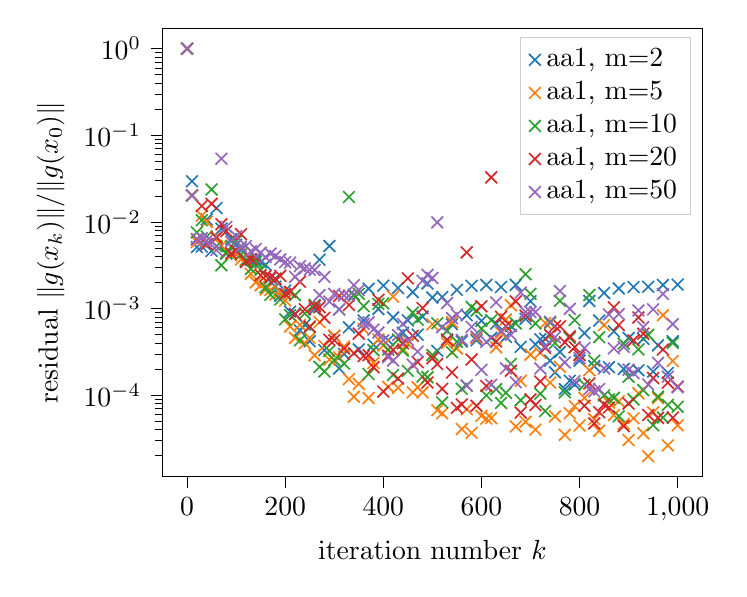
\begin{tikzpicture}

\definecolor{crimson2143940}{RGB}{214,39,40}
\definecolor{darkgray176}{RGB}{176,176,176}
\definecolor{darkorange25512714}{RGB}{255,127,14}
\definecolor{forestgreen4416044}{RGB}{44,160,44}
\definecolor{lightgray204}{RGB}{204,204,204}
\definecolor{mediumpurple148103189}{RGB}{148,103,189}
\definecolor{steelblue31119180}{RGB}{31,119,180}

\begin{axis}[
legend cell align={left},
legend style={fill opacity=0.8, draw opacity=1, text opacity=1, draw=lightgray204},
log basis y={10},
tick align=outside,
tick pos=left,
x grid style={darkgray176},
xlabel={iteration number \(\displaystyle k\)},
xmin=-50, xmax=1050,
xtick style={color=black},
y grid style={darkgray176},
ylabel={residual \(\displaystyle \norm{g(x_k)}/\norm{g(x_0)}\)},
ymin=1.15072448726461e-05, ymax=1.71866740384745,
ymode=log,
ytick style={color=black}
]
\addplot [semithick, steelblue31119180, mark=x, mark size=3, mark options={solid}, only marks]
table {%
0 1
10 0.0294332765259903
20 0.00511776195799194
30 0.0052028320326697
40 0.0106257893060954
50 0.00462814678436985
60 0.01444959786169
70 0.00836318729978025
80 0.00429995255364365
90 0.00634139811273461
100 0.00546495531726454
110 0.00478754629016707
120 0.00365402380374969
130 0.00364301525005209
140 0.00362983984694989
150 0.00342410545666742
160 0.00319878085019355
170 0.00225624546679898
180 0.00179084136933032
190 0.00140076719067598
200 0.00161594385906796
210 0.000920961064973852
220 0.00086894215774606
230 0.000559024846684917
240 0.000652285691608171
250 0.000420089813738588
260 0.000983438348093059
270 0.00366073644859502
280 0.000331295350852398
290 0.00527169364528152
300 0.000479695287039857
310 0.000203684999990965
320 0.000298713979972082
330 0.000606973342145963
340 0.00144441132244609
350 0.000337574331007949
360 0.000728587415423463
370 0.00169204442869314
380 0.00038141455531244
390 0.000987584802608142
400 0.00183939691303088
410 0.000431096282263379
420 0.000788470593800591
430 0.00172461612435972
440 0.000526038742891752
450 0.000731366209554538
460 0.00154676312591442
470 0.000499997312972136
480 0.000807788054176502
490 0.00195038464970354
500 0.0013427523154201
510 0.000325566086179985
520 0.00135646675363303
530 0.000438887795543429
540 0.000659842660360159
550 0.00164363796253176
560 0.000417845095725799
570 0.000837987119237403
580 0.00182900341334022
590 0.000431580826081627
600 0.000722827024841971
610 0.00187294003660994
620 0.000458365070197728
630 0.000670618206355064
640 0.00177293790868944
650 0.000470115925495059
660 0.000628634363825594
670 0.00187544687505389
680 0.00036229332691454
690 0.000761314911490567
700 0.00121386785107941
710 0.000385554884580424
720 0.000441014383520957
730 0.000449512152695167
740 0.000250119126504885
750 0.000183191848919381
760 0.000315716903222292
770 0.000117278601557614
780 0.000146791564584659
790 0.000133039907674584
800 0.000251144260248679
810 0.000519679866435373
820 0.00122234811998109
830 0.000216735475852696
840 0.000727153925177997
850 0.0015142421467484
860 0.0002104947681306
870 0.000546121670380544
880 0.0017063194762239
890 0.000201114586796829
900 0.000456965745984954
910 0.00177285575235256
920 0.000193937899778938
930 0.000447543375749395
940 0.00178489922564955
950 0.000187328698968345
960 0.000376421172554317
970 0.00187153459555482
980 0.000180930273409598
990 0.000419963202726229
1000 0.00189002563807666
};
\addlegendentry{aa1, m=2}
\addplot [semithick, darkorange25512714, mark=x, mark size=3, mark options={solid}, only marks]
table {%
0 1
10 0.0202183632718822
20 0.00587807373584699
30 0.0117869486208018
40 0.0100117374030811
50 0.00601239558325856
60 0.00678405973094219
70 0.00533475998376815
80 0.00446183233219464
90 0.00411397841366682
100 0.00449884856224059
110 0.0036835151104931
120 0.00361625922008136
130 0.00251657253770467
140 0.00200498276785462
150 0.00185899156300933
160 0.00165587831096072
170 0.00163712137647
180 0.00144964286035187
190 0.00153048694698381
200 0.00123852607517461
210 0.000620417318768535
220 0.00045885751466035
230 0.000649718702387417
240 0.00039801614130521
250 0.00045800004899938
260 0.000289035497928641
270 0.000699807978911779
280 0.000370968803438578
290 0.000257344903664115
300 0.00048651422072948
310 0.000273136529186958
320 0.000364215546785722
330 0.000153445845771452
340 9.58851385096858e-05
350 0.000135057684345334
360 0.00057790265399896
370 9.27846758409882e-05
380 0.000234847268411488
390 0.000441045420880869
400 0.000374708340687314
410 0.000124999279133559
420 0.00137575296269942
430 0.000121634849926212
440 0.000339666695378388
450 0.000395163161301805
460 0.000108076665621681
470 0.000123452541729143
480 0.000108029212941973
490 0.000161055073027312
500 0.000656375580074275
510 6.70511648051781e-05
520 6.18654806249559e-05
530 0.000396806160933062
540 0.000697716972794646
550 0.000345398589032528
560 4.06978918481629e-05
570 6.87886378845776e-05
580 3.68020267934187e-05
590 0.000453530406861909
600 5.7899030003423e-05
610 5.36623434851535e-05
620 5.44522384031255e-05
630 0.000357358653365676
640 0.000524503368467238
650 0.000749693554426089
660 0.00109249556589708
670 4.36195117020436e-05
680 0.000146177691962407
690 4.93334056604362e-05
700 0.000294009249227041
710 4.01111770395355e-05
720 0.000308948945523927
730 0.000681334428648069
740 0.000139893788315166
750 5.69817608957152e-05
760 0.000212791960598131
770 3.48812839201379e-05
780 6.19311886140189e-05
790 7.47171798129498e-05
800 4.47062820070073e-05
810 9.31536828365611e-05
820 0.000194403908583392
830 5.28851625262495e-05
840 3.88754024441373e-05
850 0.000643310269901998
860 8.17166354879225e-05
870 5.89193700683668e-05
880 8.5296064809442e-05
890 4.66779391962796e-05
900 3.03799757743761e-05
910 5.42792234226045e-05
920 0.000105172576936002
930 3.6415585424627e-05
940 1.97771266707076e-05
950 6.33828944441362e-05
960 9.23913159850098e-05
970 0.000837903712793134
980 2.63664757749418e-05
990 0.000247686815801542
1000 4.49783819869529e-05
};
\addlegendentry{aa1, m=5}
\addplot [semithick, forestgreen4416044, mark=x, mark size=3, mark options={solid}, only marks]
table {%
0 1
10 0.0201892231636782
20 0.00757167187440868
30 0.0104592326916681
40 0.00678916819289255
50 0.023693493094694
60 0.00523032749942933
70 0.003159531337182
80 0.00438161199213819
90 0.00520673747492217
100 0.00599211383131343
110 0.00422788224328986
120 0.00354799968997398
130 0.0028607127068191
140 0.00346186920172444
150 0.00281007062962478
160 0.00175787756301027
170 0.00144292277407089
180 0.00221793109132918
190 0.00127221243882379
200 0.000750199132979007
210 0.000840463471623151
220 0.00142969900003601
230 0.000428913453701051
240 0.000878069537511994
250 0.000609098649321259
260 0.00110171773152679
270 0.000211977583345063
280 0.000188195695628844
290 0.000324082239265966
300 0.000254278986728483
310 0.000977746460904039
320 0.0002314587719031
330 0.0193713787258504
340 0.00140809550937552
350 0.00148021359451181
360 0.00106432711145666
370 0.000175584717363595
380 0.00033088925981774
390 0.00113330234407031
400 0.00114518684084137
410 0.000335947559263134
420 0.000171563994288477
430 0.000438743613140744
440 0.000325350670292015
450 0.000190730408405737
460 0.000897353928100938
470 0.00074528023923217
480 0.000164324092034844
490 0.000160976654293897
500 0.000291042391017442
510 0.000676729589852819
520 8.24952100704829e-05
530 0.000554413800468183
540 0.000313125441636446
550 0.000413397270622586
560 0.000118542732434099
570 0.000129241134118885
580 0.00104107548248776
590 0.000947174151779599
600 0.000587524812564701
610 9.95380599717723e-05
620 0.000732739064734302
630 0.000117069206432646
640 8.13609451887618e-05
650 0.000106450437225802
660 0.000229819081510628
670 0.000674615092047289
680 8.7643266491226e-05
690 0.00249172211582454
700 0.00147925977881689
710 0.000673240154275033
720 0.000104060971445282
730 6.55046266273565e-05
740 0.000683984433676152
750 0.000400702994274661
760 0.00122994974551037
770 0.000107846409057661
780 0.000457368947511096
790 0.000736035752799168
800 0.000292823168378343
810 0.000132106709258614
820 0.00143104902710343
830 0.000249764333556414
840 0.000467348494601984
850 9.9490137174126e-05
860 8.98118413554828e-05
870 9.33780637754043e-05
880 5.72091442299927e-05
890 0.000394198946150581
900 0.000163160988736473
910 8.94334649038515e-05
920 0.000338204624549062
930 0.000114292841413643
940 0.000496892550767012
950 4.51178197107259e-05
960 9.6462569470028e-05
970 5.52081754907377e-05
980 7.73529327345741e-05
990 0.000401953823272071
1000 7.34179954548792e-05
};
\addlegendentry{aa1, m=10}
\addplot [semithick, crimson2143940, mark=x, mark size=3, mark options={solid}, only marks]
table {%
0 1
10 0.0201892229624445
20 0.00631791067062451
30 0.0152529505929428
40 0.00554207950046971
50 0.0161848165896331
60 0.0065678750001332
70 0.00941473187793649
80 0.00781260861347977
90 0.00433311560218223
100 0.00462993838493149
110 0.00721596486150885
120 0.00344404265703562
130 0.00374116680294207
140 0.0038787664163929
150 0.00243279810850584
160 0.00238053540934819
170 0.00231323495339577
180 0.00218634266127
190 0.00238619628840722
200 0.00147969882466997
210 0.00156279852913549
220 0.000859606053228335
230 0.00204070580577545
240 0.000978391118878055
250 0.000620081830599135
260 0.00106329194406009
270 0.00103820335823295
280 0.000782163016917595
290 0.000435550267358115
300 0.00042983638476772
310 0.00139888892775454
320 0.000344671792235616
330 0.00109875737980318
340 0.0003053211120976
350 0.000513410307536512
360 0.00028315714356994
370 0.000289577982987125
380 0.000210937778678747
390 0.00125870253451546
400 0.000110080074947063
410 0.000286788811611395
420 0.000332797629697585
430 0.000155730421730456
440 0.000398032486450646
450 0.00222905532312253
460 0.000484585552418159
470 0.000240814642040892
480 0.00101191093002057
490 0.00014016886093488
500 0.00026668224085429
510 0.000229413279555974
520 0.000118561001874354
530 0.000432502243014434
540 0.000182967228400681
550 7.13974440648186e-05
560 7.80809024411589e-05
570 0.00444320308569558
580 0.00025789347102008
590 7.53529247407703e-05
600 0.00106154369153973
610 0.000127590618558747
620 0.032663060734832
630 0.000416993102178227
640 0.000803445382416558
650 0.000626061883390191
660 0.00019152662154747
670 0.00121006353536726
680 6.29922424463932e-05
690 0.000826044845410292
700 8.95226778345046e-05
710 7.68076181546344e-05
720 0.000143770245572828
730 0.000351382267682464
740 0.000495629863075561
750 0.000625673649418261
760 0.000622479663677427
770 0.000407485847787348
780 0.000477442071743462
790 0.000358118425085904
800 0.000290612818966828
810 7.54754144924277e-05
820 0.000136678484549718
830 4.73237650414527e-05
840 6.37585516375557e-05
850 7.83062459287549e-05
860 7.20276168894621e-05
870 0.00103268985697689
880 0.000646284646421625
890 4.39598115498788e-05
900 8.01331950439069e-05
910 0.000429215845691276
920 0.000788516969168013
930 0.000512095023303877
940 5.91586048105985e-05
950 0.000157720487459246
960 5.47395915289182e-05
970 0.00033678684632244
980 0.000139374724810918
990 5.50246777057907e-05
1000 0.000125866044034427
};
\addlegendentry{aa1, m=20}
\addplot [semithick, mediumpurple148103189, mark=x, mark size=3, mark options={solid}, only marks]
table {%
0 1
10 0.0201892229598993
20 0.00631556245371639
30 0.00650052919923591
40 0.00606120366460124
50 0.0059504081157464
60 0.00473521351172619
70 0.0535766709157282
80 0.00875520659690845
90 0.00592761883527089
100 0.00685495432548994
110 0.0051832919244797
120 0.00525742758227729
130 0.00457791008465522
140 0.00486669771006026
150 0.00441051692617827
160 0.0039283830370862
170 0.00430430923969309
180 0.00403932190517596
190 0.00369672256374536
200 0.00343880080831067
210 0.00338940945318631
220 0.00232341142595783
230 0.00309327452660114
240 0.00291312934552046
250 0.00280636919400238
260 0.0027868087301498
270 0.00142881921303893
280 0.00231737617931857
290 0.00120312717053925
300 0.00147501445493734
310 0.000976327016913724
320 0.00142077935729148
330 0.00140893040569245
340 0.00185986095975613
350 0.0016277417814998
360 0.000666395491657173
370 0.000693623050309141
380 0.00057250431141103
390 0.000529768800670203
400 0.000429638939535622
410 0.000274123322331301
420 0.000251726417236804
430 0.00049308955379647
440 0.000665555227366922
450 0.000435296065169857
460 0.000224783761093266
470 0.000318310234699785
480 0.00209277691314966
490 0.00244741027477618
500 0.00225361698701004
510 0.00987908734704939
520 0.000608699124472425
530 0.00115831180835453
540 0.000775583842210992
550 0.000851517600345035
560 0.000435581957047546
570 0.000128988195161688
580 0.000614315716905087
590 0.000474371784201397
600 0.000196133889858649
610 0.000412610584846807
620 0.000131943040644988
630 0.00117799295518104
640 0.000551057220806674
650 0.000204015886690167
660 0.000497453646143894
670 0.000141163130556215
680 0.00152829860570382
690 0.000912609854923813
700 0.000912873930275977
710 0.000911288344705644
720 0.000203444716186169
730 0.000365553503865261
740 0.000705539451247987
750 0.000466229289096481
760 0.0015905086798405
770 0.000238688583847358
780 0.000991624685427819
790 0.000145279794585039
800 0.000267900740664077
810 0.00034950653470464
820 0.000117239667365791
830 0.000110381586512494
840 0.000117557743210676
850 0.000203556711404529
860 0.000855542904711617
870 0.000347342023060894
880 0.000863742292093837
890 0.000360655023604647
900 0.000196606862922742
910 0.000180033408730504
920 0.000951594168516553
930 0.000611374385485556
940 0.000133033455240102
950 0.000979395141343036
960 0.000236555372293682
970 0.00147359545187242
980 0.000163516673914698
990 0.000661702489662399
1000 0.000123219758458611
};
\addlegendentry{aa1, m=50}
\end{axis}

\end{tikzpicture}

%	}
%	\caption{Residual norms for the elastic net regression problem.}
%	\label{pl:memory_comparison_ISTA}
%\end{figure}
%
%In figure \ref{pl:memory_comparison_ISTA} we see how the performance of the 'aa1-safe' method depends on the memory parameter 'm'.

\subsection{Markov decision process}

In a second experiment $f$ originates from a random Markov decision process which is motivated in \cite[Section 5.1f]{ZhaAA}. Our aim is to find a fixed point of the Bellman operator
\begin{align*}
	f\colon\R^{n}\to\R^{n}, \qquad x\mapsto \brk*{\max_{a} \brk3{ R_{sa}+\gamma \sum_{s'}P_{sas'}x_{s'}}}_{s=1}^{n}
\end{align*}
with some $R\in\R^{S\times A}$, $P\in\R^{S\times A\times A}$ and $\gamma\in\R$. Here the parameter $\gamma$ determines the Lipschitz-constant of $f$. Again, we choose the parameters as in \cite[Section 5.2]{ZhaAA}. In particular we choose $n=1000$, $A=200$, $S=300$ and $A$ and $R$ to be randomly generated.

\begin{figure}
	\centering
	{\scriptsize
	% This file was created with tikzplotlib v0.10.1.
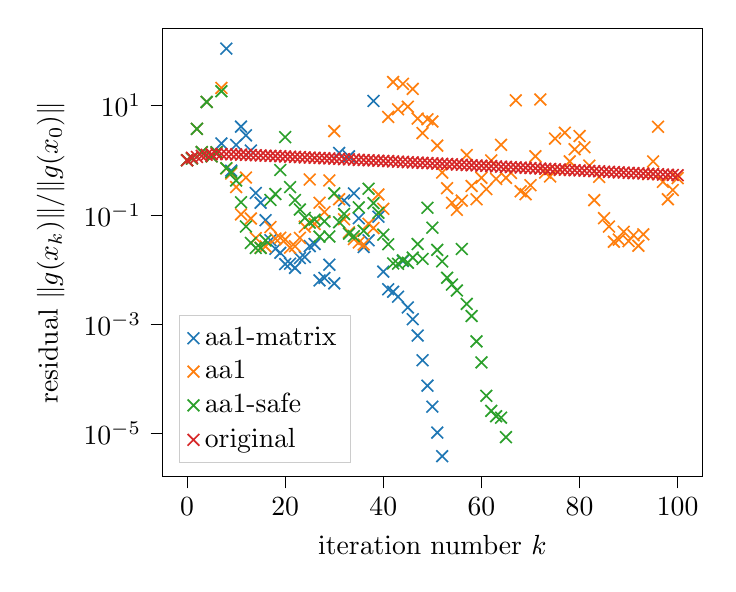
\begin{tikzpicture}

\definecolor{crimson2143940}{RGB}{214,39,40}
\definecolor{darkgray176}{RGB}{176,176,176}
\definecolor{darkorange25512714}{RGB}{255,127,14}
\definecolor{forestgreen4416044}{RGB}{44,160,44}
\definecolor{lightgray204}{RGB}{204,204,204}
\definecolor{steelblue31119180}{RGB}{31,119,180}

\begin{axis}[
legend cell align={left},
legend style={
  fill opacity=0.8,
  draw opacity=1,
  text opacity=1,
  at={(0.03,0.03)},
  anchor=south west,
  draw=lightgray204
},
log basis y={10},
tick align=outside,
tick pos=left,
x grid style={darkgray176},
xlabel={iteration number \(\displaystyle k\)},
xmin=-5, xmax=105,
xtick style={color=black},
y grid style={darkgray176},
ylabel={residual \(\displaystyle \norm{g(x_k)}/\norm{g(x_0)}\)},
ymin=1.60296195707055e-06, ymax=261.868355124713,
ymode=log,
ytick style={color=black}
]
\addplot [semithick, steelblue31119180, mark=x, mark size=3, mark options={solid}, only marks]
table {%
0 1
1 1.0755352611976
2 3.75518838234461
3 1.40628851599404
4 11.6731981104118
5 1.18093749372409
6 1.40090421673219
7 2.02605208035701
8 110.855584100498
9 0.64299179145963
10 1.91144309408162
11 4.12446814721846
12 2.85460109126495
13 1.50249666162343
14 0.251205150601463
15 0.166293114161814
16 0.0797489829230232
17 0.0342426071237798
18 0.0238054047282902
19 0.0201489019010843
20 0.0125154156840777
21 0.0127557313187956
22 0.0106679992851388
23 0.0161160416854488
24 0.0168690615217546
25 0.0267086132400852
26 0.0292336863375988
27 0.00627322825958725
28 0.00697823400058037
29 0.0121953938118291
30 0.0055394529279481
31 1.36073832068966
32 0.18328022485708
33 1.17444486198859
34 0.246282012548284
35 0.0865123016219927
36 0.025707725904967
37 0.0341585475725228
38 12.1879265954052
39 0.0923599656207338
40 0.00909908345876289
41 0.00432935914206484
42 0.00389702471232035
43 0.00315576535280723
44 0.0142448544348705
45 0.00200994763206351
46 0.00122248718286097
47 0.000613565453494968
48 0.000216476510141801
49 7.40442164113307e-05
50 3.0626535396057e-05
51 1.02496242861587e-05
52 3.78659329100655e-06
};
\addlegendentry{aa1-matrix}
\addplot [semithick, darkorange25512714, mark=x, mark size=3, mark options={solid}, only marks]
table {%
0 1
1 1.0755352611976
2 3.75518838234461
3 1.40628851599404
4 11.6731981103986
5 1.18093749372475
6 1.40090421616873
7 21.0912019324716
8 0.70870600396331
9 0.570297650356802
10 0.322529636092132
11 0.102193584174393
12 0.481435161627573
13 0.085675898504481
14 0.0374927006626434
15 0.0250260389329003
16 0.0263157380580473
17 0.0596292730513785
18 0.036670165926002
19 0.0379947327293252
20 0.0353329144480571
21 0.0249763430957848
22 0.0265886430999367
23 0.0377755277196999
24 0.0606746132878881
25 0.443266643471147
26 0.0679847432096324
27 0.166454456284775
28 0.112233327323453
29 0.426769036511151
30 3.41839726753447
31 0.193218877052916
32 0.0829595338095186
33 0.0479415193942411
34 0.0359655820658479
35 0.031067732771904
36 0.0285092780529861
37 0.0684009444779291
38 0.0571529674523425
39 0.235566886876386
40 0.128790519333626
41 6.22019290307633
42 27.116016556281
43 8.57637406894161
44 25.0449244918908
45 9.5489543004263
46 20.2402157946371
47 5.80104541557022
48 3.14229009356857
49 5.62679129805719
50 5.11292069649021
51 1.85130458736423
52 0.593255168512513
53 0.307533415590951
54 0.166277732136469
55 0.123331236768738
56 0.181640408255167
57 1.2424073292166
58 0.33777331305255
59 0.192881758501067
60 0.477374519564243
61 0.295492445661322
62 0.990574483062264
63 0.454616143397486
64 1.91129125498097
65 0.475388799565499
66 0.585056546287322
67 12.5058932929057
68 0.269674786369433
69 0.238510038163391
70 0.348737332413189
71 1.18196729070279
72 12.9723366292576
73 0.59471869542614
74 0.505013385344903
75 2.49228210835087
76 0.66327604599685
77 3.18769670756081
78 0.952123144097934
79 1.58653631488289
80 2.77484317408581
81 1.72824248833414
82 0.796674816125711
83 0.186123405568593
84 0.494955633470806
85 0.0868573782465203
86 0.0609407272606319
87 0.0320773195364773
88 0.035208635426304
89 0.048947221557114
90 0.0329580583350393
91 0.042205995800249
92 0.0271252957060362
93 0.043913152501916
94 0.554390056101532
95 0.951266625380796
96 4.1038286243902
97 0.402418275298581
98 0.192947324364005
99 0.284575966026025
100 0.469499417269773
};
\addlegendentry{aa1}
\addplot [semithick, forestgreen4416044, mark=x, mark size=3, mark options={solid}, only marks]
table {%
0 1
1 1.0755352611976
2 3.75518838234461
3 1.40628851599404
4 11.6731981103986
5 1.18093749372475
6 1.40090421616873
7 18.3456530314188
8 0.715148295715168
9 0.603184874497339
10 0.425000949481369
11 0.169780826096162
12 0.0610485339134772
13 0.0305596317163464
14 0.024662407440244
15 0.0246382815657975
16 0.0338590603309514
17 0.186686880407098
18 0.240877438483814
19 0.661480487236913
20 2.65067879029495
21 0.321999702180161
22 0.186511288485043
23 0.125389579384999
24 0.0878772233638788
25 0.0718833450727415
26 0.081494558422746
27 0.0397308140326577
28 0.0761026889423139
29 0.0401036223462444
30 0.247509959435394
31 0.0731889916720187
32 0.103585298565059
33 0.045086682627828
34 0.0407133723461978
35 0.136980200139006
36 0.0509839251598084
37 0.300554295464308
38 0.163465459395862
39 0.108988183598972
40 0.043327709663486
41 0.0289227145257426
42 0.0128813285858401
43 0.0126860573907805
44 0.0146564454574554
45 0.01325974161395
46 0.0164604751045286
47 0.0291452089847411
48 0.015590365896841
49 0.134695639629952
50 0.0581346749350764
51 0.0228054942020384
52 0.0140334060162714
53 0.00703327472488363
54 0.00528226336165501
55 0.00411214985737699
56 0.0236594230889657
57 0.0023297129844864
58 0.00140091505531589
59 0.000480811027458525
60 0.000197776724896766
61 4.82833971743053e-05
62 2.56094179453485e-05
63 2.04171816953548e-05
64 1.92083011769677e-05
65 8.45279620283931e-06
};
\addlegendentry{aa1-safe}
\addplot [semithick, crimson2143940, mark=x, mark size=3, mark options={solid}, only marks]
table {%
0 1
1 1.11079595696464
2 1.15146347935386
3 1.19810871768358
4 1.25836079969792
5 1.28717661562128
6 1.29872016999624
7 1.29969634748056
8 1.29427780315209
9 1.28581920504604
10 1.27622052601559
11 1.26611180186867
12 1.25567973744064
13 1.24515860112889
14 1.23464410447634
15 1.22475614752878
16 1.21456170949969
17 1.20395648888282
18 1.19328571131099
19 1.18239771328136
20 1.1716325696414
21 1.16090350150878
22 1.15045593968254
23 1.13986574349194
24 1.13013419365196
25 1.1205532570567
26 1.11009686004258
27 1.09942016181751
28 1.08888621792244
29 1.07846836032938
30 1.06812180776554
31 1.05797103677549
32 1.04767742392812
33 1.03756456334062
34 1.02745332608267
35 1.01759036852571
36 1.00792809955725
37 0.998740205929624
38 0.989307642541083
39 0.979662513131675
40 0.970013642411032
41 0.960333158618473
42 0.950896200427626
43 0.941587432298908
44 0.932314052853465
45 0.92303520246954
46 0.913827971469853
47 0.904718177964474
48 0.89569530853438
49 0.886740378504046
50 0.877873881691319
51 0.869095416833083
52 0.860404577532346
53 0.851800574188502
54 0.84328258562761
55 0.834849767218491
56 0.826589259756341
57 0.8183311439405
58 0.810152200452982
59 0.802099498877686
60 0.794119851883925
61 0.786190328690046
62 0.778330775381482
63 0.770548406416384
64 0.762843504933984
65 0.755215418730901
66 0.747663417653967
67 0.740231629489046
68 0.732890752171026
69 0.725595792718312
70 0.718363555481887
71 0.711191150771091
72 0.704082221187788
73 0.69704258049511
74 0.690072684660852
75 0.683172292051206
76 0.676340683573591
77 0.669577324728221
78 0.662881574090997
79 0.656252769324686
80 0.649690246573462
81 0.64319334620614
82 0.636761413630057
83 0.630393799857749
84 0.6240898620134
85 0.617848963461753
86 0.611670473856904
87 0.605553769131258
88 0.599498231445486
89 0.593503249133445
90 0.58756821664316
91 0.581692534477183
92 0.575875609132603
93 0.570116853041361
94 0.564415684510987
95 0.558771527665891
96 0.55318381238924
97 0.547651974265354
98 0.542175454522701
99 0.536753699977473
100 0.531386162977699
};
\addlegendentry{original}
\end{axis}

\end{tikzpicture}

	}
	\caption{Residual norms for the Markov decision process problem.}
	\label{pl:method_comparison_VI}
\end{figure}

The performance for the various methods can be seen in figure \ref{pl:method_comparison_VI}. In contrast to the other methods the the 'aa2-matrix' method does not converge here. In this problem the fixed point iteration ('original') converges very slowly. The 'aa1-safe' method outperforms all others. This confirms numerically that the 'aa1-safe' algorithm can deal with the problems it was specifically designed for and for which the fixed point iteration fails to converge in adequate time. 

\begin{figure}
	\centering
	{\scriptsize
	% \tiny
	% This file was created with tikzplotlib v0.10.1.
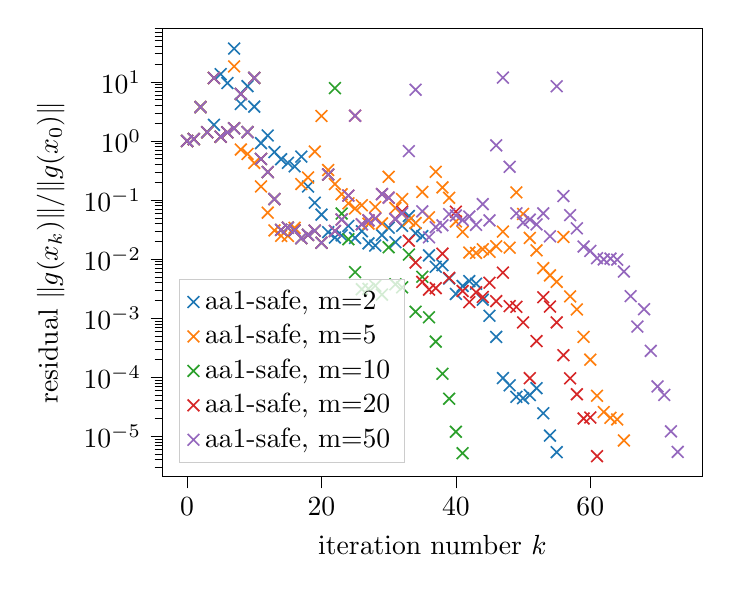
\begin{tikzpicture}

\definecolor{crimson2143940}{RGB}{214,39,40}
\definecolor{darkgray176}{RGB}{176,176,176}
\definecolor{darkorange25512714}{RGB}{255,127,14}
\definecolor{forestgreen4416044}{RGB}{44,160,44}
\definecolor{lightgray204}{RGB}{204,204,204}
\definecolor{mediumpurple148103189}{RGB}{148,103,189}
\definecolor{steelblue31119180}{RGB}{31,119,180}

\begin{axis}[
legend cell align={left},
legend style={
  fill opacity=0.8,
  draw opacity=1,
  text opacity=1,
  at={(0.03,0.03)},
  anchor=south west,
  draw=lightgray204
},
log basis y={10},
tick align=outside,
tick pos=left,
x grid style={darkgray176},
xlabel={iteration number \(\displaystyle k\)},
xmin=-3.65, xmax=76.65,
xtick style={color=black},
y grid style={darkgray176},
ylabel={residual \(\displaystyle \norm{g(x_k)}/\norm{g(x_0)}\)},
ymin=2.06939624145893e-06, ymax=81.2659656416253,
ymode=log,
ytick style={color=black}
]
\addplot [semithick, steelblue31119180, mark=x, mark size=3, mark options={solid}, only marks]
table {%
0 1
1 1.0755352611976
2 3.75518838234461
3 1.40628851599404
4 1.87853063613969
5 13.5683039394205
6 9.58061673888226
7 36.7048898816999
8 4.24661402743947
9 8.48817637310083
10 3.82063487989049
11 0.920670350537736
12 1.23927765977764
13 0.649253059430202
14 0.490428196043484
15 0.426276801870825
16 0.371867570126604
17 0.543449995355047
18 0.169382002599128
19 0.0899676945022177
20 0.0564864518621158
21 0.0285638686557645
22 0.0231629633841192
23 0.0251714415732592
24 0.0364682613614003
25 0.022784673891762
26 0.0296184697515113
27 0.0184569438636945
28 0.0169172772180602
29 0.0254526759277122
30 0.034043316054264
31 0.0193022548131288
32 0.036498280577338
33 0.0536128322463297
34 0.0274074875752158
35 0.0244737265394726
36 0.011528388424917
37 0.00739831395049804
38 0.0078765991309671
39 0.00467128132924836
40 0.00256277056176505
41 0.00349475076026708
42 0.0042345176335238
43 0.00382053859903931
44 0.00205005484633863
45 0.00109488301187244
46 0.000479189832706216
47 9.62470726573469e-05
48 7.25518182039349e-05
49 4.63754009112666e-05
50 4.39443021466736e-05
51 4.96463698873923e-05
52 6.50480766217488e-05
53 2.44280257386611e-05
54 1.02303715573834e-05
55 5.35408849999778e-06
};
\addlegendentry{aa1-safe, m=2}
\addplot [semithick, darkorange25512714, mark=x, mark size=3, mark options={solid}, only marks]
table {%
0 1
1 1.0755352611976
2 3.75518838234461
3 1.40628851599404
4 11.6731981103986
5 1.18093749372475
6 1.40090421616873
7 18.3456530314188
8 0.715148295715168
9 0.603184874497339
10 0.425000949481369
11 0.169780826096162
12 0.0610485339134772
13 0.0305596317163464
14 0.024662407440244
15 0.0246382815657975
16 0.0338590603309514
17 0.186686880407098
18 0.240877438483814
19 0.661480487236913
20 2.65067879029495
21 0.321999702180161
22 0.186511288485043
23 0.125389579384999
24 0.0878772233638788
25 0.0718833450727415
26 0.081494558422746
27 0.0397308140326577
28 0.0761026889423139
29 0.0401036223462444
30 0.247509959435394
31 0.0731889916720187
32 0.103585298565059
33 0.045086682627828
34 0.0407133723461978
35 0.136980200139006
36 0.0509839251598084
37 0.300554295464308
38 0.163465459395862
39 0.108988183598972
40 0.043327709663486
41 0.0289227145257426
42 0.0128813285858401
43 0.0126860573907805
44 0.0146564454574554
45 0.01325974161395
46 0.0164604751045286
47 0.0291452089847411
48 0.015590365896841
49 0.134695639629952
50 0.0581346749350764
51 0.0228054942020384
52 0.0140334060162714
53 0.00703327472488363
54 0.00528226336165501
55 0.00411214985737699
56 0.0236594230889657
57 0.0023297129844864
58 0.00140091505531589
59 0.000480811027458525
60 0.000197776724896766
61 4.82833971743053e-05
62 2.56094179453485e-05
63 2.04171816953548e-05
64 1.92083011769677e-05
65 8.45279620283931e-06
};
\addlegendentry{aa1-safe, m=5}
\addplot [semithick, forestgreen4416044, mark=x, mark size=3, mark options={solid}, only marks]
table {%
0 1
1 1.0755352611976
2 3.75518838234461
3 1.40628851599404
4 11.6731981104185
5 1.18093749372393
6 1.40090421692276
7 1.63964739059953
8 6.26598610287106
9 1.41332552898251
10 11.7034275047632
11 0.495347115413464
12 0.297708556049388
13 0.103854919243168
14 0.0312147680982529
15 0.0340461055287938
16 0.0305455749722938
17 0.0225946209431041
18 0.0256738797707145
19 0.0301855160087205
20 0.018856463716004
21 0.270629103387766
22 7.85523539060093
23 0.0589406036320235
24 0.0216123404840444
25 0.00601103163824777
26 0.00308603501951992
27 0.0031235241976028
28 0.0035249549594548
29 0.00249956787203374
30 0.0158337686993174
31 0.00373768056664869
32 0.00331335424021668
33 0.0118978115773371
34 0.00128124039546379
35 0.00500826139208636
36 0.00103195123238441
37 0.000398906056018016
38 0.00011415701190929
39 4.3017788148578e-05
40 1.18698860701722e-05
41 5.14430465103244e-06
};
\addlegendentry{aa1-safe, m=10}
\addplot [semithick, crimson2143940, mark=x, mark size=3, mark options={solid}, only marks]
table {%
0 1
1 1.0755352611976
2 3.75518838234461
3 1.40628851599403
4 11.6731981103978
5 1.18093749372495
6 1.40090421613532
7 1.63964738889284
8 6.26598612000159
9 1.41332552384319
10 11.7034275337047
11 0.495347138133032
12 0.297708580231871
13 0.103854933468859
14 0.0312147684103382
15 0.0340461050170883
16 0.0305455759100881
17 0.0225946213779845
18 0.0256738768594627
19 0.0301855341349567
20 0.0188564953159085
21 0.270629907124791
22 0.0298763370447055
23 0.04665461337723
24 0.118721335726454
25 2.67716778625344
26 0.038797807782173
27 0.0451151649174011
28 0.0485603277561161
29 0.125846077872067
30 0.109496298149191
31 0.047681200856897
32 0.0635936603971914
33 0.0204465108546445
34 0.00871547143267722
35 0.00409407268904007
36 0.00304000372593451
37 0.00321895531538506
38 0.0123253874615148
39 0.00479469830911402
40 0.0635274517678392
41 0.00287278004861663
42 0.0018633989647495
43 0.00273489183265452
44 0.00227557973845975
45 0.00396881908354306
46 0.00193240971737209
47 0.00588982055014076
48 0.00159483828868021
49 0.00154877928456481
50 0.000845035512841143
51 9.60037797002976e-05
52 0.000407361161560409
53 0.00225410343374082
54 0.00156792685442704
55 0.000845020375651434
56 0.000234794429083028
57 9.53436693137172e-05
58 5.12740693080488e-05
59 1.99114170611133e-05
60 2.07037647234824e-05
61 4.5817187954882e-06
};
\addlegendentry{aa1-safe, m=20}
\addplot [semithick, mediumpurple148103189, mark=x, mark size=3, mark options={solid}, only marks]
table {%
0 1
1 1.0755352611976
2 3.75518838234461
3 1.40628851599403
4 11.6731981103978
5 1.18093749372491
6 1.40090421613089
7 1.63964738888369
8 6.26598612010074
9 1.41332552381866
10 11.7034275319982
11 0.495347138884487
12 0.297708581022815
13 0.103854933927618
14 0.0312147684225771
15 0.0340461050099375
16 0.0305455759443623
17 0.0225946213885691
18 0.0256738767725365
19 0.0301855347117061
20 0.0188564963160158
21 0.270629932518448
22 0.0298763368546127
23 0.0466546142343731
24 0.118721361011239
25 2.67716787517599
26 0.0387978069342984
27 0.0451151648853361
28 0.048560327882539
29 0.12584609764353
30 0.109496313427667
31 0.0476812069731635
32 0.059773559877093
33 0.673886524107571
34 7.38097781491731
35 0.0642558386456773
36 0.0233511512274654
37 0.0347604733489515
38 0.037293020272592
39 0.0576834913838587
40 0.0547362824562971
41 0.0458044595810415
42 0.0525276670784326
43 0.0379348316132706
44 0.0851463573017842
45 0.0451829309251776
46 0.843433319453169
47 11.8362627581299
48 0.365110522081558
49 0.0594663066007335
50 0.0415430162082251
51 0.0465952588428236
52 0.0385627204481566
53 0.0593605827836918
54 0.024287636013756
55 8.44687625363979
56 0.116738133251526
57 0.0554101775100425
58 0.033150720822543
59 0.0162916079520256
60 0.0137403985667986
61 0.0103358226843191
62 0.0098802457341439
63 0.0101701475560081
64 0.00975828372466841
65 0.00614828310464411
66 0.0023541583850147
67 0.00071799813130963
68 0.00141280352417749
69 0.000279013771129767
70 6.95897200347232e-05
71 4.98818286257152e-05
72 1.20567813827281e-05
73 5.40980630651396e-06
};
\addlegendentry{aa1-safe, m=50}
\end{axis}

\end{tikzpicture}

	}
	\caption{Residual norms for the Markov decision process problem.}
	\label{pl:memory_comparison_VI}
\end{figure}

In figure \ref{pl:memory_comparison_VI}  we see how the performance of the 'aa1-safe' method depends on the memory parameter $m$. In particular one sees that the algorithm performs best for this problem with a parameter of $m\approx10$. We also see that increasing the parameter $m$ does not necessarily improve performance of the method as in this plot the choice $m=50$ performs worst.

\newpage

\section{Summary}

The AA-I algorithm is specifically tailored to find the fixed point of a function $f$ which is expensive to evaluate, noisy, has an unknown gradient and where the dimension $n$ is large. The main idea of the AA-I and AA-II algorithms is to generalise the fixed point iteration by setting $x_{k+1}=\sum_i\alpha_if_i$ for some clever choice of $\alpha=\alpha^k\in\R^{k+1}$. The AA-I algorithm one obtains requires some modifications. More specifically, one applies Powell-type regularisation and a restarting of the iteration for well-definedness. One builds in a mechanism for safeguarding of the steps for convergence and one uses a rank-1 update formula to make the implementation matrix-free. One can then show the convergence of the algorithm under the assumption that $f$ is non-expansive and that there exists a fixed point. The numerical experiments then show that the AA-I algorithm with the modifications outperforms the fixed point iteration for the problems tested.



\section*{Bibliography}
\nocite{*}
Main source
\printbibliography[heading=none, keyword={main}]
\noindent Other sources
\printbibliography[heading=none, keyword={secondary}]

\end{document}
